% ===========================================================================
% BEFORE SUBMITTING: read SUBMISSION_REQUIREMENTS.md in this directory.
% It contains the full checklist, anonymity steps, desk-rejection risks,
% and the contribution-acknowledgement directive from the program chairs.
% ===========================================================================
% SUBMISSION TOGGLE: set \showchecklisttrue before uploading to OpenReview.
\newif\ifshowchecklist
\showchecklisttrue   % <-- change to \showchecklistfalse to hide during drafting

\documentclass{article}

% NeurIPS 2026 style: download neurips_2026.sty from the NeurIPS submission site
% Options: (none) = anonymous submission, [final] = camera-ready, [preprint] = arXiv
\usepackage[eandd]{neurips_2026}

\usepackage[T1]{fontenc}
\renewcommand{\ttdefault}{lmtt}  % LM mono for listings; keeps NeurIPS text font
\usepackage{microtype}
\usepackage{graphicx}
\usepackage{subcaption}
\usepackage{booktabs}
\usepackage{tabularx}
\usepackage{hyperref}
\usepackage{enumitem}
\usepackage{amsmath}
\usepackage{amssymb}
\usepackage{mathtools}
\usepackage{amsthm}
\usepackage{caption}
\usepackage{tcolorbox}
\usepackage{array}
\usepackage{colortbl}
\usepackage{ragged2e}
\usepackage{listings}
\usepackage{pifont}
\usepackage{dblfloatfix}  % enables [b] placement for figure* in two-column mode
\usepackage{afterpage}   % \afterpage defers figure* to top of next page
\IfFileExists{savetrees.sty}{\usepackage[subtle]{savetrees}}{}

% Relax float placement
\renewcommand{\bottomfraction}{0.55}
\renewcommand{\textfraction}{0.10}
\renewcommand{\floatpagefraction}{0.7}
\setcounter{bottomnumber}{2}
\setcounter{topnumber}{2}
\setcounter{totalnumber}{4}

% ── Syntax-highlighted Python listings ────────────────────────────────────────
\definecolor{codekw}{HTML}{5B21B6}      % violet  — keywords
\definecolor{codestr}{HTML}{0F766E}     % teal    — strings / docstrings
\definecolor{codecmt}{HTML}{6B7280}     % gray    — comments
\definecolor{codedec}{HTML}{B45309}     % amber   — decorators (@)
\definecolor{codecls}{HTML}{1D4ED8}     % blue    — class names

\lstset{
  language=Python,
  basicstyle=\scriptsize\ttfamily,
  breaklines=true,
  columns=flexible,
  keepspaces=true,
  showstringspaces=false,
  keywordstyle=\color{codekw}\bfseries,
  commentstyle=\color{codecmt}\itshape,
  stringstyle=\color{codestr},
  % decorators: colour from @ to end of line
  moredelim=[l][\color{codedec}\bfseries]{@},
  % underscore fix: render as proper text underscore, not math subscript
  literate={_}{{\textunderscore}}1,
  % highlight key class names as blue
  emph={Task, Tool, Benchmark, BenchmarkConfig, TaskConfig,
        ToolConfig, CompositeBenchmarkConfig, WorkArenaConfig,
        WebArenaVerifiedConfig, MiniWoBConfig, WebTask, BrowserTool,
        Observation},
  emphstyle=\color{codecls},
}

% ── Experiment placeholders: update these once results are locked ─────────────
\newcommand{\NUMCUBES}{10}            % registered CUBEs at submission
\newcommand{\NUMEXP}{8}               % CUBEs used in experiments
\newcommand{\NUMMODELS}{4}            % frontier models evaluated
\newcommand{\NUMTASKS}{2{,}100}       % unique tasks across the experimental corpus
\newcommand{\TOPRESULT}{65.1\%}       % best per-CUBE pass rate (Sonnet 4.6, SWE-bench Verified)

% Compact paragraph-style heading: bold inline, small leading skip.
\newcommand{\mypar}[1]{\par\noindent\textbf{#1}\enspace}

% Standard error suffix in tables: smaller, gray, with leading thinspace.
% Use as: 42.2 \SE{4.2}  →  42.2 ±4.2 (smaller, muted gray)
\newcommand{\SE}[1]{\,{\scriptsize\textcolor{gray!70}{$\pm$#1}}}
\newcommand{\NA}{\textcolor{gray!60}{---}}   % model did not run this benchmark

\newcommand{\cmark}{\ding{51}}
\newcommand{\xmark}{\ding{55}}
\newcommand{\pmark}{$\sim$}

\definecolor{rowalt}{HTML}{F8FAFC}

% ===========================================================================
% STYLE GUIDE FOR ALL SECTIONS (read before drafting any section)
% ===========================================================================
% DO NOT USE em dashes (---). Use commas, parentheses, periods, or colons.
% Avoid common AI-generated tells:
%   - "delve", "moreover", "furthermore", "in conclusion", "it is worth noting"
%   - "tapestry", "landscape" as filler, "navigate" as a verb for ideas
%   - "comprehensive", "holistic", "robust" as throwaway adjectives
%   - "leverage" (use "use"), "utilize" (use "use")
%   - opening sentences that begin with "In recent years" or "With the advent of"
%   - paragraphs that summarize what the paragraph just said
%   - bulleted lists where prose would be tighter
% Prefer concrete claims over hedged ones. Cite specific numbers from
% experiments rather than "significant improvements". Active voice.
% Short sentences are fine. One idea per sentence is fine.
%
% ANONYMITY: Do not cite the CUBE position paper (arxiv-only, would
% de-anonymize). The NeurIPS paper must be self-contained on the standard.
% ===========================================================================

\title{CUBE: A Unified Standard and Benchmark Suite for Evaluating Generalist Agents}

% Author block: hidden automatically in anonymous submission mode.
% Switch to \usepackage[final]{neurips_2026} for camera-ready to reveal.
% NOTE: NVIDIA authors (Frujeri, Cuevas, Memarian, Mayorga, Zhang) pending
%       internal review approval before final submission.
\author{%
  \textbf{Alexandre Lacoste}$^{1}$ \quad
  \textbf{Nicolas Gontier}$^{1}$ \quad
  Oleh Shliazhko$^{1}$ \quad
  Aman Jaiswal$^{1,3}$ \quad
  Kusha Sareen$^{1,6,7}$ \quad
  Shailesh Nanisetty$^{1}$ \quad
  Joan Cabezas \quad
  Manuel Del Verme$^{2}$ \quad
  Omar G.\ Younis$^{2}$ \quad
  Simone Baratta$^{2}$ \quad
  Matteo Avalle$^{2}$ \quad
  Imene Kerboua$^{7}$ \quad
  Xing Han L\`{u}$^{6,7}$ \quad
  Felipe Vieira Frujeri$^{4}$ \quad
  Marc Cuevas$^{4}$ \quad
  Farzan Memarian$^{4}$ \quad
  Natasha Mayorga$^{4}$ \quad
  Vivienne Zhang$^{4}$ \quad
  Elron Bandel$^{4}$ \quad
  Michal Shmueli-Scheuer$^{4}$ \quad
  Asaf Yehudai$^{4}$ \quad
  Leshem Choshen$^{4}$ \quad
  Jonathan Lebensold$^{5}$ \quad
  Sean Hughes$^{1}$ \quad
  Massimo Caccia$^{1}$ \quad
  Alexandre Drouin$^{1,7}$ \quad
  Siva Reddy$^{6,7}$ \quad
  Tao Yu$^{8}$ \quad
  Yu Su$^{9}$ \quad
  Graham Neubig$^{10}$ \quad
  Dawn Song$^{11}$ \\[6pt]
  \small
  $^{1}$ServiceNow AI Research \quad
  $^{2}$Silverstream.ai \quad
  $^{3}$Dalhousie \quad
  $^{4}$IBM Research \quad
  $^{5}$Jetty \\
  $^{6}$McGill University \quad
  $^{7}$Mila -- Quebec AI Institute \quad
  $^{8}$HKU \quad
  $^{9}$OSU \quad
  $^{10}$CMU \quad
  $^{11}$UC Berkeley \\
  The AI Alliance \\[4pt]
  \texttt{alexandre.lacoste@servicenow.com} \quad \texttt{nicolas.gontier@servicenow.com}
}

\begin{document}

\maketitle
\enlargethispage{1.5cm}

\begin{abstract}
The agentic benchmark landscape now exceeds 600 environments and is
still growing, yet each one ships its own provisioning logic, action
space, tool definitions, and evaluation harness. The resulting
$N\times M$ integration tax blocks cross-benchmark research,
including the multi-environment RL post-training that recent work
identifies as the strongest path to generalist capability.
We introduce \textbf{CUBE} (Common Unified Benchmark Environments): a
Python-first standard for tasks, benchmarks, tools, and a three-tier
resource lifecycle, with an optional JSON-RPC interface for non-Python
clients. Any runtime that drives the \texttt{Task} gym API is a valid
harness; AgentBeats and NeMo Gym already consume CUBE benchmarks.
The reference harness adds auto-provisioning across Docker, VM, and
live backends, a registry of \NUMCUBES{} wrapped benchmarks across
web, computer-use, SWE, and terminal modalities, and a trajectory
judge that attributes per-episode failures to agent, tool, or
benchmark causes via $K{=}3$ cross-judging with post-hoc evidence
verification.
We evaluate \NUMMODELS{} frontier models on \NUMEXP{} CUBEs with tool
stacks held constant per modality, exposing capability profiles that
per-benchmark leaderboards do not surface and pinpointing where
failures live: roughly 82\,\% trace to the LLM itself, with the rest
concentrating on specific tool stacks and on wrapper bugs that the
judge surfaces and that we then fix in place. Wrapping a new
benchmark reduces to a few typed classes plus metadata, and a Claude
skill turns even that into an afternoon of work.
\end{abstract}


% ===========================================================================
\section{Introduction}
\label{sec:intro}
% \afterpage defers this full-width figure to the top of page 2 so the
% NeurIPS submission notice stays at the bottom of page 1 by itself.
\afterpage{%
\begin{figure*}[t!]
  \centering
  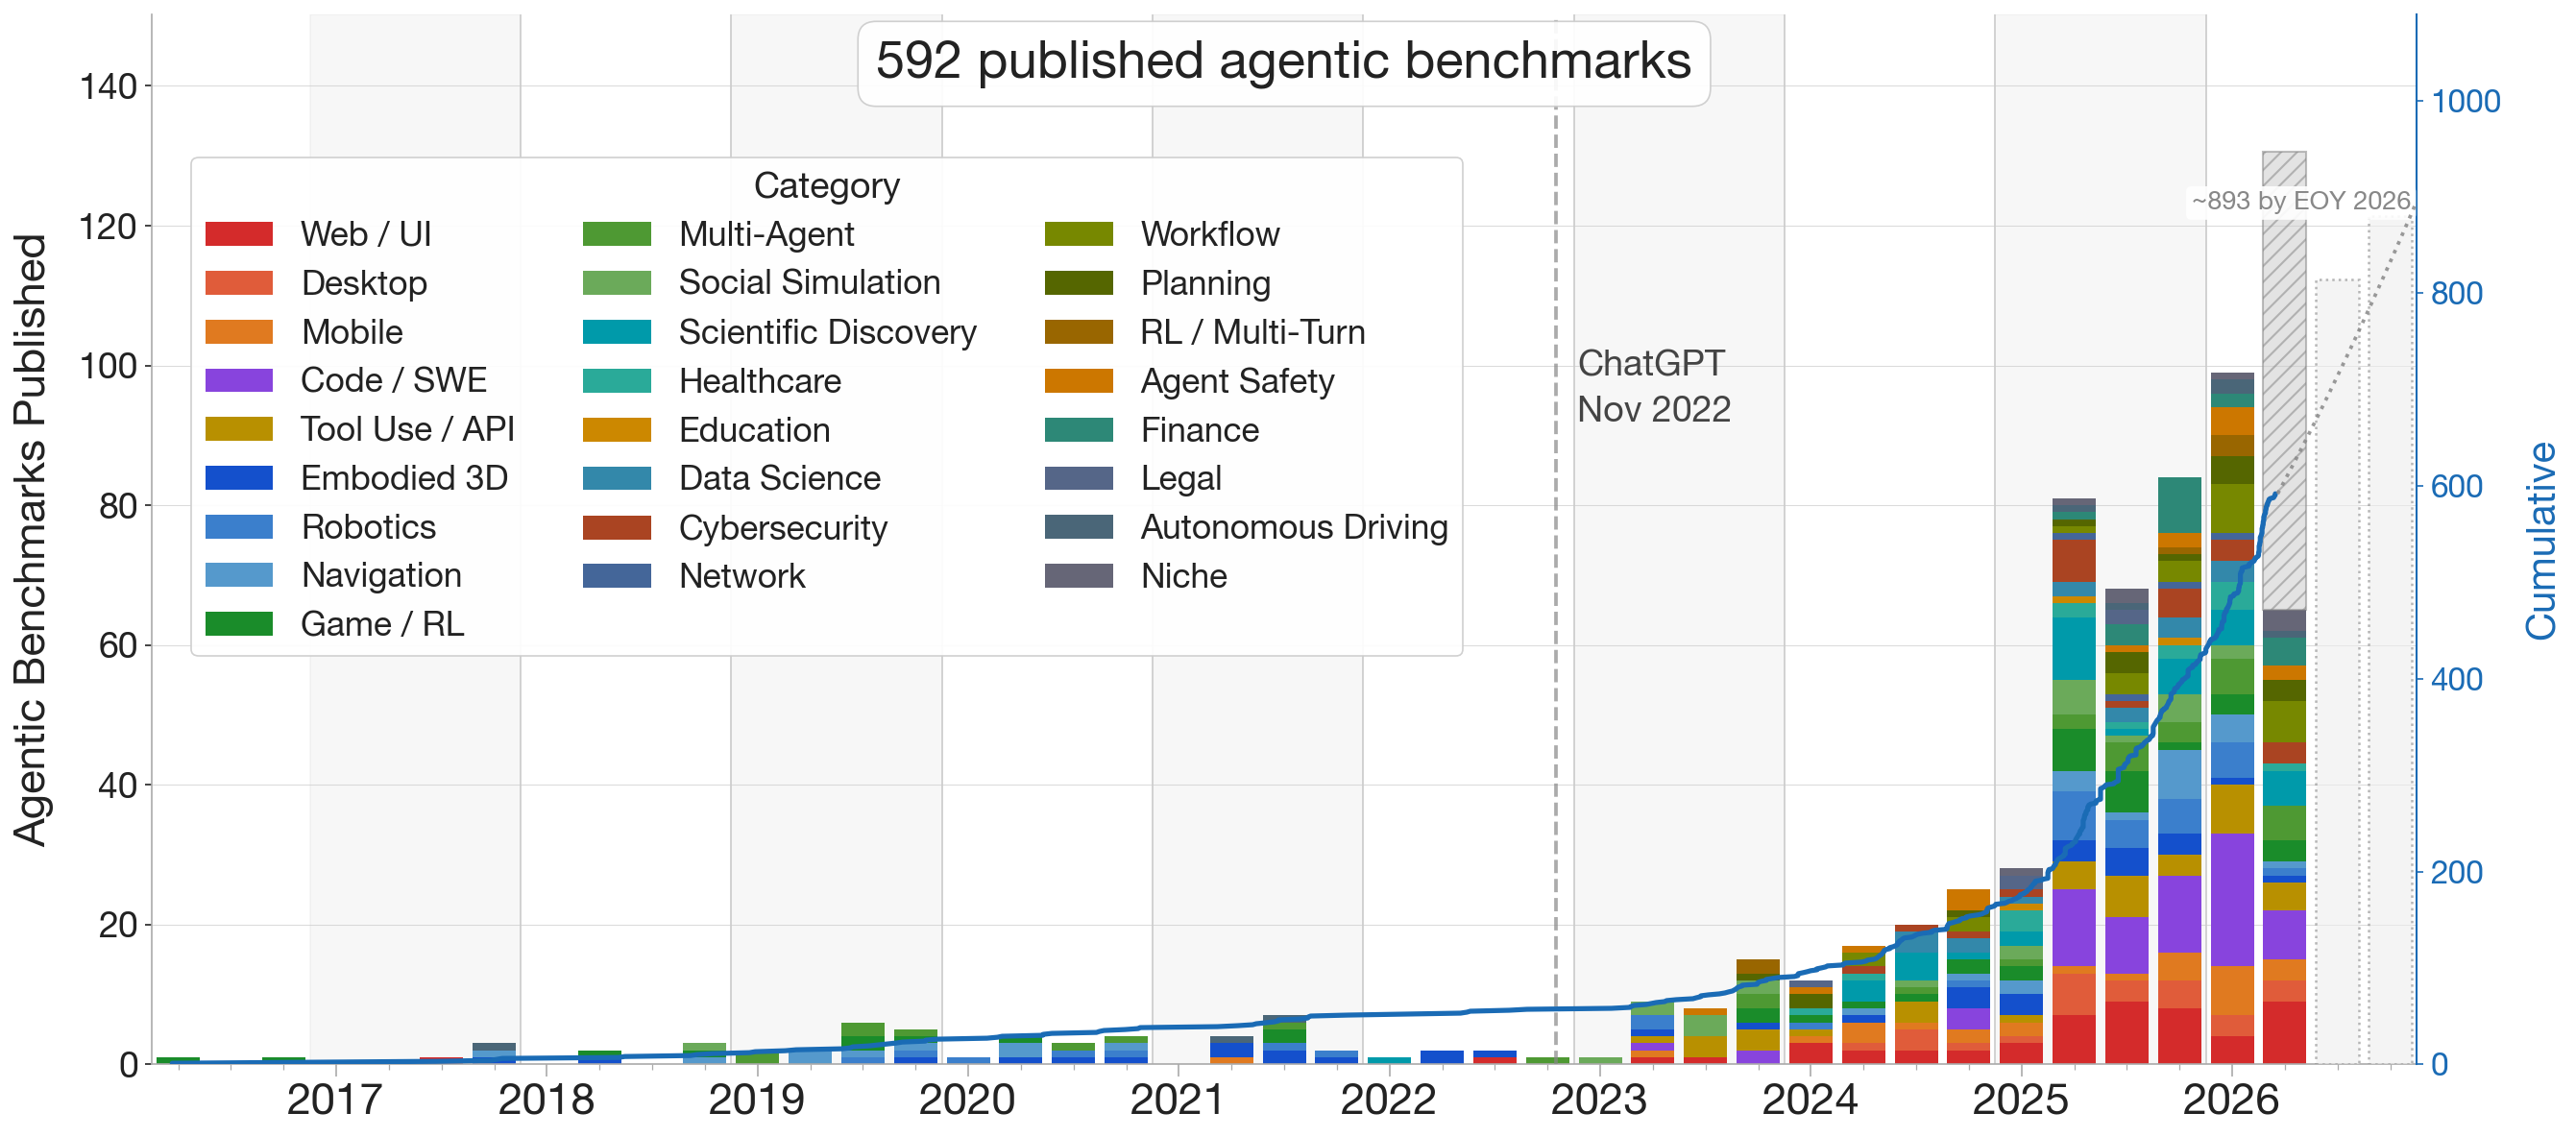
\includegraphics[width=\linewidth]{figures/benchmarks_timeline.png}
  \caption{
    Agentic benchmarks published per quarter, 2016--2026, by category
    (cumulative count on right axis).
    Dashed line: ChatGPT (November 2022).
    Q2~2026 is ${\approx}37\%$ complete; the gray hatched bar estimates remaining
    Q2 publications from a monthly linear trend since January~2023.
    Outlined bars and dotted projection line show Q3--Q4~2026 forecasts from the
    same model. See \S\ref{sec:corpus} for corpus details.
  }
  \label{fig:timeline}
\end{figure*}%
}
% ===========================================================================
% LENGTH TARGET: 1.25-1.5 pages including Figure 1.
%
% PARAGRAPH 1 (the explosion): The agentic benchmark landscape has gone
% from a handful of environments to 600+ in tree years and is still
% accelerating. Reference Figure 1 (the timeline plot, n=592 from our
% landscape analysis through April 2026, forecasting ~1100 by EOY).
% Drop-in number: "X new agentic benchmarks were published in Q1 2026
% alone" (use 100 from our data).
%
% PARAGRAPH 2 (the integration tax): Each benchmark ships its own
% scaffolding: bespoke action spaces, harness assumptions, provisioning
% scripts, evaluation harnesses. A team that wants to evaluate one agent
% on five benchmarks pays five integration costs. This is the bottleneck
% the field has not yet named. State plainly.
%
% PARAGRAPH 3 (the frontier framing, kept tight): Multi-environment RL
% post-training is now demonstrably the strongest known route to
% generalist capability gains (cite Nemotron-3 Super or equivalent
% public result with concrete number). But that paradigm depends on
% sampling tasks across many environments at scale. Without a shared
% network interface and resource lifecycle, curriculum-style training across
% benchmarks is impractical. The integration tax is not just an
% engineering nuisance; it is what holds the next frontier back.
%
% PARAGRAPH 4 (contributions, numbered list with one sentence each):
%   1. The CUBE Standard: a Python-first set of abstractions for tasks,
%      benchmarks, tools, and resources, with a JSON-RPC interface option.
%   2. A reference harness with auto-provisioning across Docker, VM,
%      and live backends; the standard is harness-agnostic and
%      interoperates with AgentBeats and NeMo Gym.
%   3. A corpus of 10-12 wrapped CUBEs across 4 modalities, with a
%      live registry and automated 2-tier compliance verification.
%   4. CUBE-Composite: a 15-line class for building cross-benchmark
%      composites, instantiated as a difficulty-calibrated composite
%      benchmark.
%   5. The first systematic cross-modality evaluation of frontier
%      models with tooling held constant per modality.
%
% PARAGRAPH 5 (forward-looking framing, weave in but do NOT promise
% sections that do not exist): Briefly mention that standardization
% enables three lines of follow-on research: (a) tools as an
% independent variable across benchmark families, (b) composite
% benchmarks that evolve as agents improve, (c) curriculum-driven
% generalist training. We discuss these as concrete directions in
% Section 8 anchored to the experimental findings.
%
% FIGURE 1 (must appear in or just after this section):
%   - The benchmarks_timeline_paper.png (n=592, ChatGPT marker,
%     forecast bars). Caption emphasizes: agentic benchmarks since
%     2017, exponential since ChatGPT, 600+ today, 1100+ forecast EOY
%     2026, color-coded by category, n=592 from our manual review.
%   - This is THE motivation figure. Make the caption do narrative work.

The number of agentic benchmarks has grown from a handful to over 600 in five years
(Figure~\ref{fig:timeline}). More than 100 new benchmarks were published in Q1 2026 alone,
spanning web navigation, computer use, software engineering, embodied control, scientific
discovery, and a dozen other categories.\footnote{%
  Corpus curated via deep search of arxiv listings; each entry requires an interactive
  environment, links to a published paper, and has been individually verified.}
This growth reflects genuine scientific demand: agentic evaluation is hard, domain coverage
is uneven, and researchers keep finding gaps that require new environments. The
proliferation is a sign of health, not pathology. The problem is that each benchmark
arrives as an island, shipping its own scaffolding.

WebArena requires a set of web servers
provisioned from a specific snapshot. SWE-bench requires per-task Docker containers cloned
from a repository matrix. OSWorld requires a pre-provisioned virtual machine image with a
running desktop. WorkArena requires a live ServiceNow instance. Every benchmark defines its
own action space, names its own tools, makes its own assumptions about how an agent is
called, and provides its own (often fragile) evaluation harness. A team that wants to
evaluate a single agent across five benchmarks pays five independent integration costs.
The cost multiplies with models: $N$ models on $M$ benchmarks means $N \times M$
integration points. No wonder cross-benchmark results are rare and comparisons are almost
always informal.

This fragmentation blocks more than evaluation. Recent work argues that future agentic
systems should be designed for generality across diverse environments
\citep{bandel2026agentic}, and large-scale reinforcement learning post-training has emerged
as a primary route to capability gains in frontier models \citep{Khatri2025TheAO}: every
additional environment the model trains on adds a dimension of generalization it could not
acquire from any one benchmark alone.
With 600+ agentic benchmarks now in existence, the ideal training curriculum already exists
on paper. But sampling from hundreds of environments at training time requires every
benchmark to expose the same interface, the same resource lifecycle, and the same tool
vocabulary. No such interface exists today. Every custom integration is a constraint on
the training distribution, and a narrower distribution caps what can be learned.
The integration tax on evaluation is the ceiling on generalist capability tomorrow.

We introduce \textbf{CUBE} (Common Unified Benchmark Environments), addressing this bottleneck through four contributions.
\mypar{The CUBE Standard (Section~\ref{sec:standard}):} a Python-first set of abstractions for tasks, benchmarks, tools, and resources, with a three-tier resource lifecycle for transparent auto-provisioning across Docker, VM, and cloud backends, and an optional JSON-RPC interface for non-Python clients. The standard also introduces a composite benchmark class that subsets and combines existing CUBEs as a difficulty-calibrated cross-modality benchmark.
\mypar{A reference harness (Section~\ref{sec:harness}):} although the standard is harness-agnostic and interoperates with AgentBeats and NeMo Gym, we provide a reference harness with parallel execution, OpenTelemetry tracing, trajectory logging for RL training data, and a trajectory judge that attributes per-episode failures to agent, tool, or benchmark causes, making cross-benchmark failure analysis tractable at scale.
\mypar{A wrapped corpus and registry (Section~\ref{sec:corpus}):} \NUMCUBES{} CUBEs spanning web, computer use, software engineering, and terminal modalities, with automated compliance verification and a live registry. At the time of writing the registry includes a cube for MiniWoB \citep{Shi2017WorldOB}, WebArena \citep{zhou2024webarena}, WorkArena \citep{drouin2024workarena}, BrowseComp \citep{wei2025browsecomp}, OSWorld \citep{xie2024osworld}, Windows Agent Arena \citep{bonatti2025windows}, SWE-bench \citep{jimenez2023swebench}, SWE-bench Verified \citep{yang2024swebenchverified}, Terminal-Bench \citep{merrill2026terminalbenchbenchmarkingagentshard}, and DRBench \citep{abaskohi2025drbench}; and with the release of our claude skill to wrap any benchmark within CUBE, we expect the registry to grow significantly.
% \mypar{CUBE-Composite (Section~\ref{sec:composite}):} a first-class composite benchmark class that subsets and combines existing CUBEs in roughly 15 lines of Python; we instantiate it as a difficulty-calibrated cross-modality benchmark.
\mypar{Cross-modality evaluation (Section~\ref{sec:experiments}):} a systematic evaluation of frontier models across web, CUA, and SWE tasks with tooling held constant per modality, exposing capability profiles that per-benchmark reports tend to miss.

Standardization enables research that is otherwise impractical. When tools are first-class objects in the standard, tool design becomes an independent variable: one browser tool drives WebArena, WorkArena, and MiniWoB, making tool ablations honest across benchmark families.
When composites are a core abstraction, difficulty can be recalibrated as agents improve without re-engineering anything. 
When every benchmark speaks the same interface, curriculum training across hundreds of environments is a sampling-policy decision, not an integration project.
% Section~\ref{sec:discussion} returns to each with evidence.


% ===========================================================================
\section{Related Work}
\label{sec:related}
% ===========================================================================

\paragraph{Agentic benchmarks.}
The agent-evaluation landscape now spans hundreds of environments
\citep{yehudai2025surveyevaluationllmbasedagents}, including
multi-environment benchmarks such as AgentBench
\citep{Liu2023AgentBenchEL}, AppWorld \citep{appworld2024}, and
$\tau$-bench \citep{taubench2024}; each individual benchmark CUBE
wraps embeds strong infrastructure assumptions.
WebArena \citep{zhou2024webarena} requires a persistent shared server stack;
WorkArena \citep{drouin2024workarena} requires a live ServiceNow instance;
OSWorld \citep{xie2024osworld} and Windows Agent Arena \citep{bonatti2025windows}
require VM snapshots with a running desktop;
SWE-bench \citep{jimenez2023swebench,yang2024swebenchverified} creates per-task Docker
containers from a repository matrix;
Terminal-Bench \citep{merrill2026terminalbenchbenchmarkingagentshard} uses hermetic
per-task containers; MiniWoB \citep{Shi2017WorldOB} runs inside a local browser.
These incompatible resource models are the direct source of the $N \times M$ integration
tax described in Section~\ref{sec:intro}.
BrowserGym \citep{chezelles2025browsergym} demonstrates the value of a shared interface
within the web modality; CUBE generalizes this approach across modalities and lifts
the benchmark interface to include resource provisioning and tool configuration.
HAL \citep{kapoor2025holisticagentleaderboardmissing} surfaces a complementary problem:
without controlled tooling, scores on the same benchmark are not comparable across papers.
CUBE addresses this directly by making tools first-class objects in the standard, so
the tool configuration is part of the benchmark's declared interface.

\paragraph{Platforms and orchestration.}
Several systems address agentic evaluation and training from complementary angles.
The METR Task Standard \citep{metr_task_standard_2024} fixes a portable Docker/VM task-image convention with a small lifecycle of hooks; $\sim$200 task families have been wrapped under it, and it is used across METR, UK AISI, and partner organizations.
Inspect AI \citep{inspect_ai} is AISI's evaluation orchestration framework, with 200+ pre-built evaluations, sandboxing, MCP \citep{mcp2024} tool support, and bridges to coding agents.
AgentGym \citep{xi2025agentgym} bundles 14 environments under a unified HTTP API, primarily as substrate for its AgentEvol training method rather than as a third-party-extensible standard.
AgentBeats \citep{agentbeats2025} proposes the Agentified Agent Assessment paradigm, in which benchmarks are realized as judge agents communicating over A2A and MCP, and operates a registry of judge agents alongside hosted competitions.
NeMo Gym \citep{nemo-gym} provides high-throughput RL training infrastructure with a microservice architecture and integrations into NeMo RL and OpenRLHF; OpenEnv \citep{openenv2025} distributes Gymnasium-style environments through the HuggingFace Hub.
PipelineRL \citep{piche2025pipelinerl} streams weight updates to inference workers to overlap generation and training on long-trajectory rollouts, and Harbor \citep{Shaw_Harbor_Framework_2025} grew out of Terminal-Bench as a container-based post-training pipeline.

These systems operate at distinct layers: image conventions (METR), evaluation orchestration (Inspect), curated training suites (AgentGym), and RL execution (the rest). CUBE sits at the wrapping layer with a Python-native typed object model for tasks, benchmarks, tools, and the resource lifecycle, a JSON-RPC contract for non-Python clients, a registry for third-party contributions, and reference connectors that expose any CUBE benchmark as a NeMo Gym environment or an AgentBeats green agent.

\paragraph{RL post-training over agentic environments.}
Reinforcement learning post-training is now central to frontier LLM development and
follows predictable scaling laws \citep{Khatri2025TheAO}; recent position work argues that
the natural endpoint is generalist agentic systems trained and evaluated across diverse
environments \citep{bandel2026agentic}. Prior work on multi-environment RL for agents
has been limited to bespoke per-project integrations, with custom reset and reward logic
per environment and no shared tool vocabulary. A standard task interface, resource
lifecycle, and portable tool set are the precondition layer that makes large-scale
curriculum training across heterogeneous benchmarks tractable rather than a per-project
engineering effort.


% ===========================================================================
\section{The CUBE Standard}
\label{sec:standard}
% ===========================================================================

The CUBE standard serves two audiences. A \emph{downstream user} (a harness,
a training platform, or a researcher) needs to run any benchmark and provision its resources through a single uniform interface, without writing benchmark-specific code.
A \emph{benchmark author} needs a clear contract so that a single CUBE compliant implementation reaches all downstream users at once.
The standard is harness-agnostic and ships as a pure Python library.\footnote{%
  Anonymous repository: \url{https://anonymous.4open.science/r/cube-standard-123}}
A central design principle is the \emph{config/make split}: every runtime
object (benchmark, task, tool) has a serializable config counterpart that
crosses process boundaries safely; calling \texttt{.make()} on the config
returns the live object that holds a dynamic state and is never serialized.

% ── 3.1 ──────────────────────────────────────────────────────────────────────
\subsection{Running a CUBE}
\label{sec:standard-user}

Running a CUBE is config-first. A downstream user assembles an experiment by composing serializable Python objects: a tool config, a benchmark config, an infra config, and an agent config.
The framework separates shared setup from per-task execution: calling \texttt{.make(infra)} on the benchmark config provisions shared resources (servers, containers, VMs) once; the resulting task configs are lightweight serializable records that travel to Ray workers, which access or instantiate live environments locally based on their needs.
Only serializable handles, (endpoints, IDs, infra config) cross to worker processes via a \texttt{runtime\_context} dict, never live environments. Workers access live clients locally from those handles.
The episode loop (right box) is gym-style: observe, act, repeat until terminal.
The key addition over vanilla Gymnasium~\citep{towers2024gymnasium} is that \texttt{evaluate()} is decoupled from \texttt{step()} and can be called at any point independently of action frequency, which matters when agent and evaluator run on different schedules.

\vspace{-5pt}
\noindent
\begin{minipage}[t]{0.48\columnwidth}
\vspace{0pt}%
{\scriptsize\centering\textbf{Harness side:} configure, iterate, dispatch\par\vspace{-5pt}}
\begin{tcolorbox}[colback=blue!3, colframe=blue!25, arc=2mm,
  boxrule=0.5pt, left=2mm, right=0mm, top=1mm, bottom=0.5mm, boxsep=0pt]
\begin{lstlisting}[basicstyle=\tiny\ttfamily, aboveskip=0pt, belowskip=0pt]
# serializable configs defines the experiment
tool_cfg = BrowsergymConfig(use_screenshot=True)
wav_cfg = WebArenaVerifiedConfig(tool_config=tool_cfg)
agent_cfg = MyAgentConfig(llm_config=...)
infra_cfg = AzureInfraConfig()  # or AWS, GCP, local

@ray.remote
def run(task_cfg, runtime_ctx, agent_cfg):
  # right box -->
  return run_episode(task_cfg, runtime_ctx, agent_cfg)

# .make() provisions shared resources
# leaving the 'with' block tears them down
with wav_cfg.make(infra_cfg) as bench:
  rc = bench.runtime_context  # endpoints, IDs, infra
  task_cfgs = bench.config.get_task_configs()
  ray.get([run.remote(tc, rc, agent_cfg) for tc in task_cfgs])
\end{lstlisting}
\end{tcolorbox}  
\end{minipage}
\hfill
\begin{minipage}[t]{0.48\columnwidth}
\vspace{0pt}
{\scriptsize\centering\textbf{Gym-like Episode loop:} one task, one agent\par\vspace{2pt}}
\begin{tcolorbox}[colback=blue!3, colframe=blue!25, arc=2mm,
  boxrule=0.5pt, left=2mm, right=0mm, top=1mm, bottom=0.5mm, boxsep=0pt]
\begin{lstlisting}[aboveskip=0pt, belowskip=0pt]
# evaluation running on a remote process
def run_episode(task_cfg, runtime_ctx, agent_cfg):
    task  = task_cfg.make(runtime_ctx)
    agent = agent_cfg.make(task.action_set)
    obs, _ = task.reset()
    done = False
    while not done:
        act = agent.act(obs)
        out = task.step(act)
        obs, done = out.obs, out.done
    return task.evaluate()
\end{lstlisting}
\end{tcolorbox}
\end{minipage}
%\medskip

\mypar{Resource provisioning.}
A benchmark declares its infrastructure requirements as a list of \texttt{ResourceConfig}: the base image its containers or VMs need, any storage volumes, and setup scripts.
When an experiment starts, the harness resolves these against the user's \texttt{InfraConfig}, downloads the original benchmark artifacts, and builds or registers a benchmark-ready image on the target provider (local Docker, Azure, AWS, or others).
Benchmark authors write their \texttt{ResourceConfig} once; users point at any supported infra target and benchmark code does not change.
Three structurally different provisioning patterns appear across the corpus:
(i) WebArena needs a shared server started once per run: the author starts it in
\texttt{Benchmark.\_setup()} and passes the URL to tasks via \texttt{RuntimeContext};
(ii) SWE-bench needs a fresh container per task: the harness launches one via \texttt{runtime\_context['infra']} when the task is constructed.
(iii) OSWorld needs a pre-built VM image: the author declares a \texttt{VMResourceConfig}; the harness builds it on first use and caches it.

\mypar{Composite benchmarks and RPC interface.}
\texttt{CompositeBenchmarkConfig} composes any number of existing benchmarks into a single standards-compliant one. Task IDs are prefixed by sub-benchmark name; routing is transparent to callers. Provisioning, RPC server, compliance verification, and registry metadata are all inherited. Composites nest freely.
The standard also auto-generates a JSON-RPC~2.0 server with MCP-compatible endpoints from any \texttt{Benchmark} subclass, so any MCP client drives a CUBE task without an adapter layer (see Appendix~\ref{apdx:json-rpc-protocol}).

% ── 3.2 ──────────────────────────────────────────────────────────────────────
\subsection{Wrapping a Benchmark}
\label{sec:standard-author}

Every CUBE must provide a default tool that defines the agent's action space:
the tool is the benchmark's public interface for any downstream agent or
training pipeline, so tool selection is the first authoring decision.
The standard ships reusable reference tools for each major modality.
A BrowserGym-compatible browser tool drives web benchmarks (WebArena,
WorkArena, MiniWoB); a desktop tool built on accessibility trees and
PyAutoGUI drives CUA benchmarks (OSWorld, Windows Agent Arena); terminal
tools drive SWE and scripted benchmarks.
For benchmarks where tool design is itself a research variable, the separation
between tool and task means a benchmark ships a sensible default while staying
configurable: swapping the tool for the same benchmark produces directly
comparable scores because the environment is held constant.
Once a tool is chosen, authoring reduces to three steps: (1) declare benchmark metadata, task metadata and
resources; (2) implement \texttt{reset()} and \texttt{evaluate()} on the Task subclass, and (3) ship a debug suite.

\mypar{Tools.}
Custom tools follow the \texttt{@tool\_action} pattern: the
decorator derives the full action schema from the method signature and
docstring, so no separate specification is needed.
\texttt{ToolConfig.make(container)} instantiates the tool after its container
is live; switching to a different backend means swapping the \texttt{InfraConfig} passed to \texttt{.make(infra)}; tool, task and benchmark code are unchanged.

\mypar{Metadata and task execution info.}
A benchmark declares \texttt{BenchmarkMetadata} (name, version, description,
task count, reset isolation mode) and per-task \texttt{TaskMetadata} (id, split, container config). Heavy per-task data (patches, archives, long problem statements, binaries) lives on a \texttt{TaskExecutionInfo} subclass populated lazily on workers, keeping initialization flat at scale.
\texttt{BenchmarkConfig.install()} writes that data to a per-task cache (\texttt{\$HOME/.cube/...}) once per worker; later runs read it from disk.

\mypar{Evaluation.}
\texttt{task.evaluate()} is the benchmark author's primary scientific contribution.
It returns a reward in $[0,1]$ with a structured info dict.
The base class calls it at episode end, but the harness can also call it
independently to support partial-credit scoring or judge-agent analysis.
Privileged evaluation data (ground-truth patches, evaluator scripts, internal state) lives in the \texttt{task.execution\_info} field, kept off the agent's observation and tool surface; an opt-in \texttt{task.get\_privileged\_info()} hook exposes it to judge agents or debug clients when needed.

\mypar{Debug suite and robustness.}
Every CUBE ships two LLM-free contracts that the standard requires and the compliance check verifies.
\texttt{get\_debug\_benchmark()} returns a \texttt{BenchmarkConfig} pre-filtered
to a small set of tasks with deterministic, known-correct solutions.
\texttt{make\_debug\_agent(task\_id)} returns a scripted agent guaranteed to reach reward~1.0 on those tasks without calling any language model.
Running the debug suite against real infrastructure proves that the provisioning pipeline, tool execution, and evaluation logic all work end-to-end, with no model-in-the-loop ambiguity.
The registry runs this suite post-merge whenever an entry changes; the result feeds the entry's status badge on the registry site.
Locally, \texttt{cube test <name>} runs the same suite, so authors catch broken environments before pushing.

\mypar{Authoring tools.}
The standard ships with layer-by-layer specifications in \texttt{openspec/specs/};
each spec includes Invariants and Gotchas sections that enumerate the most common
authoring mistakes.
Two Claude Code skills exploit these specifications directly.
\texttt{/new-cube} generates a complete CUBE package from a benchmark description:
task subclass, tool subclass, benchmark subclass, debug suite, serializable configs,
and \texttt{pyproject.toml}, all consistent with the standard's invariants.
\texttt{/review-cube} audits an existing implementation against those invariants
and reports violations before the registry's compliance check runs.
These skills are the primary onboarding path for new contributors and reduce
the typical wrapping effort for an existing benchmark from days to hours.

% ===========================================================================
\section{A Reference Harness}
\label{sec:harness}
% ===========================================================================

The CUBE standard is harness-agnostic: any runtime that can instantiate a
\texttt{BenchmarkConfig} and drive the \texttt{Task} gym API is a valid
harness. AgentBeats and NeMo Gym both consume CUBE benchmarks directly,
and a reference NeMo Gym connector in \texttt{cube-standard} exposes any
benchmark as a Gymnasium environment for RL frameworks in roughly 100 lines\footnote{\href{https://anonymous.4open.science/r/cube-standard-123/src/cube/integrations/nemogym.py}{https://anonymous.4open.science/r/cube-standard-123/src/cube/integrations/nemogym.py}}.
We provide a reference harness that runs the full stack end-to-end and serves
as the execution engine for the experiments in Section~\ref{sec:experiments}.
Adopting CUBE does not require adopting our harness.
The harness contributes three pieces: a generalist agent, a Ray-based
experiment runner with trajectory logging, and a trajectory judge that
automates per-episode failure analysis.

\mypar{Generalist agent.}
\texttt{Genny}, the agent used for the experiments in
Section~\ref{sec:experiments}\footnote{\href{https://anonymous.4open.science/r/cube-harness-123/src/cube_harness/agents/genny.py}{https://anonymous.4open.science/r/cube-harness-123/src/cube\_harness/agents/genny.py}},
consumes any CUBE-compliant action set without per-benchmark code and
offers two cache-friendly context modes. In \emph{growing-history}
mode, each step appends one (observation, action) pair to a stable
cacheable prefix; we use this for SWE agents, where tool-call results
themselves carry the state the agent needs to retain. In
\emph{rolling-summary} mode, a separate summarizer LLM produces a
per-step summary stored as its own message; the prompt keeps the
accumulated summaries plus the current observation while older raw
observations are dropped, so the prefix cache extends cleanly across
steps. This mode covers UI-based agents (web, CUA), where retaining
every screenshot or accessibility tree would exhaust the context
window within a few steps.

\mypar{Experiment runner.}
The runner schedules episodes with Ray. Each worker receives a serialized \texttt{Episode} (containing \texttt{TaskConfig}, \texttt{AgentConfig}, and the benchmark's \texttt{runtime\_context}), calls \texttt{make()} locally to instantiate the live task, tool, and agent, runs the episode, and ships a \texttt{Trajectory} back to the coordinator.
No live object crosses a process boundary.
The \texttt{Benchmark} itself stays on the driver.
The coordinator enforces per-step timeouts and retries transient failures (\texttt{FAILED}, \texttt{CANCELLED}, \texttt{STALE}), tracking each episode through \texttt{QUEUED}~$\to$~\texttt{RUNNING}~$\to$~\texttt{COMPLETED}|\texttt{FAILED}.
Parallelism is bounded by infra capacity and the Ray worker pool.

Trajectories are persisted to a per-episode file store that feeds RL
post-training pipelines, and LiteLLM token counts give the cost-per-task
figures used in Section~\ref{sec:experiments}.

\subsection{Trajectory judge}
\label{sec:judge}

Binary pass/fail tells you how often an agent fails, not why. With
experiments running hundreds of episodes across multiple modalities, manual
failure triage does not scale. As a remedy, the harness ships a per-episode judge that
runs an external coding agent (Claude Code via \texttt{claude-agent-sdk})
over the recorded trajectory and emits a structured \texttt{JudgeOutput}:
narrative analysis, outcome, primary blame category with confidence,
additional blames, supporting evidence, and a failure hypothesis.
Beyond diagnosing agent limitations, the blame distribution serves a second
role: it validates wrapper faithfulness. A low benchmark-side blame rate
(\texttt{env\_failure}, \texttt{eval\_brittle}, \texttt{task\_unclear})
is evidence that the CUBE wrappers are not introducing systematic
evaluation artifacts.

LLM-as-judge \citep{zheng2023judging,li2024llmjudgesurvey} remains
unreliable in general: judges underperform on objectively-correct
response comparisons \citep{tan2025judgebench}, hallucinate evidence
and miscalibrate confidence \citep{jung2025trustorescalate}, and
naive judges systematically misclassify agent-trajectory outcomes
\citep{lu2025agentrewardbench}. Closer to our setting, MAST \citep{cemri2025mast} derived a
14-mode failure taxonomy for multi-agent traces with
$\kappa{=}0.88$ agreement; the CUBE judge takes the same
evidence-grounded approach at the single-agent level, with a
3-bucket attribution into agent, tool, or benchmark causes designed
for use as a corpus-wide faithfulness signal across a
\NUMCUBES{}-benchmark suite.

\mypar{Grounded inputs.}
Per experiment, an Opus-class agent runs once (turn budget 80) to
assemble a \emph{context pack}: pointers and summaries for the agent
prompt, tool definitions, task description, reward function, and
infra entrypoints. A Sonnet-class judge then runs per episode (turn
budget 40) with the context pack and the trajectory directory,
invoked through \texttt{claude-agent-sdk}. Crucially, the judge reads
files via its own tool loop rather than receiving a stuffed prompt,
so attributions are grounded in real source: it can open a specific
step's accessibility tree or read the actual reward function.

\mypar{Constrained outputs and reliability checks.}
The judge selects the \emph{primary blame} from a fixed 10-category
taxonomy (Appendix~\ref{apdx:judge-schema}) and reports \texttt{none}
rather than inventing a cause; any non-\texttt{none} blame must be
supported by step-indexed verbatim quotes pulled from the trajectory,
and confidence is reported on a 0--5 scale. Two reliability layers
sit on top. First, \emph{post-hoc evidence verification}: every quote
is checked against the persisted step file, mismatches (literal or
fuzzy) trigger a confidence downgrade and catch the most common
hallucination mode in our setting (synthesising a plausible-looking
quote). Second, \emph{cross-judging with $K=3$}: independent judges
vote, the modal blame is reported, and quantitative aggregation is
restricted to judgements with at least two-of-three agreement after
verification. In practice $\geq 97\,\%$ of episodes reach
majority agreement on the primary blame after this filter
(Appendix~\ref{apdx:judge-meta}); transcripts are persisted with
each episode record, leaving the remaining disputed cases auditable.


% ===========================================================================
\section{Benchmark Corpus and Registry}
\label{sec:corpus}
% ===========================================================================

Our initial corpus spans web automation (WorkArena, WebArena-Verified,
MiniWoB, BrowseComp), computer use (OSWorld, Windows Agent Arena),
software engineering and terminal (SWE-bench Verified, SWE-bench Live,
Terminal-Bench), and enterprise research (DRBench), totalling 5{,}642
tasks across four structurally distinct provisioning models (local
browser, shared multi-service Docker stack, per-task Docker container,
virtual machine, and live external service). The set was assembled to
stress the standard from every direction: each modality forces a
different combination of action space, infrastructure, and evaluation
logic, and covering them in one corpus is what surfaced the abstractions
in Sections~\ref{sec:standard} and~\ref{sec:harness}. For the experiments
in Section~\ref{sec:experiments} we draw from the eight CUBEs in the Web,
CUA, and SWE blocks; BrowseComp and DRBench are omitted to keep compute
tractable. Per-CUBE task counts and backend details are tabulated in
Appendix~\ref{apdx:bench-details}.

\mypar{A registry for a decentralized corpus.}
Any author can publish a CUBE in their own repository and ship it through
any Python index. The registry is a lightweight file-based metadata index,
GitHub-orchestrated rather than a hosted service\footnote{registry URL kept private during reviewing}. Each entry is a small YAML
record (name, version, authors, license, package link) submitted via pull
request; the registry stores no benchmark code, only the pointer to a repository implementing that specific CUBE.

\mypar{Automated compliance on submission.}
Submitting a CUBE triggers GitHub Actions compliance checks. A
\emph{quick check} (schema validation, package import, action introspection)
runs on every PR in roughly two minutes. A \emph{full check} post-merge
executes the debug agent on the debug task set; a CUBE is compliant only if
the agent reaches reward~1.0 on every debug task. Passing both earns a
compliance badge; failing the full check flags the entry degraded until a
fix is submitted. This lets the registry accept third-party CUBEs at scale
without trusting any individual submitter.


% ===========================================================================
\section{Experiments}
\label{sec:experiments}
% ===========================================================================

Our experiments answer three questions.
First, can a single generalist agent configuration produce useful baselines
across the corpus (\S\ref{sec:exp-baselines})?
Second, where do its failures originate: the LLM, the agent scaffolding,
the tool stack, or the wrapped benchmark itself (\S\ref{sec:exp-judge-results})?
Third, and most critically for an evaluation suite: are the CUBE wrappers
faithful implementations of the underlying benchmarks? Reproducing published
leaderboard numbers proved too noisy a signal for this purpose
(Appendix~\ref{apdx:reproducibility}); we used the judge's benchmark-side
blame rate instead, which enabled iterative wrapper debugging and yielded
direct evidence of faithfulness once benchmark-side blame converged to a
low share.

% --- 7.1 Setup -------------------------------------------------------------
\subsection{Setup}
\label{sec:exp-setup}

\mypar{Models.}
We evaluate four frontier models spanning two providers, with a small/large
split per provider: Anthropic Claude Haiku and Claude Sonnet, OpenAI
GPT-5.4-mini and GPT-5.4. All calls go through the harness's LiteLLM gateway with
default sampling parameters.

\mypar{Agent.}
We use Genny (\S\ref{sec:harness}) as the single generalist agent across
the corpus. Genny operates in two modes selectable per benchmark: rolling
summaries for UI-based tasks (web, CUA), where retaining every screenshot or
accessibility tree would saturate the context window; growing history for
SWE and terminal tasks, where tool-call results carry the state the agent
needs to retain. We do not tune a per-benchmark prompt; the only
benchmark-aware choices are the context-management mode and the registered
tool stack.

\mypar{Tool stacks.}
One tool stack per modality, held constant across all benchmarks in that
modality. Web: BrowserGym's high-level action set. CUA:
accessibility-tree input with PyAutoGUI for action output. SWE: a bash tool
with structured stdout/stderr capture. Holding tooling constant per
modality is what lets per-modality results be compared directly across
benchmarks.

\mypar{Benchmark subsets.}
We use full sets where tractable. WorkArena is restricted to L1 and L2
(L3 omitted); SWE-bench Live \citep{zhang2025swebenchlive} to \emph{lite-gold-226}, the
lite-split tasks whose gold patches pass evaluation verbatim;
BrowseComp and DRBench are excluded. Subset sizes appear in
Table~\ref{tab:passrate}.

\mypar{Reporting.}
For each (model, CUBE) pair we report pass rate as the primary metric,
average number of steps, and average dollar cost per task as secondary
metrics. Cost is computed from token counts recorded by the LiteLLM
callback multiplied by published model rates. Each task is hard-capped at
150 steps and at a per-task budget of \$1 (small models: Haiku~4.5,
GPT-5.4-mini) or \$3 (large models: Sonnet~4.6, GPT-5.4). Tasks that
exhaust either limit are counted as failures.

\mypar{Faithfulness validation.}
We use the judge's benchmark-side blame rate as the primary
faithfulness signal: when \texttt{env\_failure}, \texttt{eval\_brittle},
and \texttt{task\_unclear} are rare, the wrapper is not the bottleneck.
This signal drove several rounds of wrapper debugging before the final
runs, each round flagging a specific evaluator error, provisioning issue,
or tool misconfiguration that we then fixed
(Appendix~\ref{apdx:reproducibility}).


% --- 6.3 Baseline pass rates -----------------------------------------------
\subsection{Baseline pass rates}
\label{sec:exp-baselines}

Table~\ref{tab:passrate} reports per-model, per-CUBE pass rate across
the subsets defined above.
%
\begin{table}[t]
\centering
\caption{Pass rate (\%) per model and CUBE on the evaluation subsets.
Best per row is shown in bold.}
\label{tab:passrate}
\small
\setlength{\tabcolsep}{5pt}
\renewcommand{\arraystretch}{1.05}
\begin{tabular}{lrcccc}
\toprule
& & \multicolumn{2}{c}{\textbf{Anthropic}} & \multicolumn{2}{c}{\textbf{OpenAI}} \\
\cmidrule(lr){3-4} \cmidrule(lr){5-6}
\textbf{CUBE (subset)} & \textbf{\# Tasks} & \textbf{Haiku 4.5} & \textbf{Sonnet 4.6} & \textbf{GPT-5.4-mini} & \textbf{GPT-5.4} \\
\midrule
WorkArena L1                    & $33{\times}10$ & 31.7\,\SE{2.6} & \textbf{65.6\,\SE{2.6}} & 27.3\,\SE{2.5} & 53.6\,\SE{2.7} \\
WorkArena L2                    & 235 & 15.6\,\SE{2.4} & \textbf{35.5\,\SE{3.1}} & 5.2\,\SE{1.4}  & 35.7\,\SE{3.1} \\
WebArena-Verified               & 381 & \NA             & \textbf{14.8\,\SE{1.8}} & \NA             & 9.0\,\SE{1.5}  \\
MiniWoB                         & $125{\times}5$ & \textbf{67.2\,\SE{1.9}} & 59.4\,\SE{2.0} & 52.5\,\SE{2.0} & 52.5\,\SE{2.0} \\
\midrule
OSWorld (PyAutoGUI)             & 360 & 43.2\,\SE{2.6} & \textbf{49.4\,\SE{2.6}} & 17.3\,\SE{2.0} & 28.6\,\SE{2.4} \\
OSWorld (Computer13)            & 360 & 42.1\,\SE{2.6} & \textbf{51.6\,\SE{2.6}} & 27.5\,\SE{2.4} & 30.7\,\SE{2.4} \\
Win.\ Agent Arena (PyAutoGUI)  & 154 & 41.5\,\SE{4.0} & \textbf{61.2\,\SE{3.9}} & 25.7\,\SE{3.5} & 37.5\,\SE{3.9} \\
Win.\ Agent Arena (Computer13) & 154 & \textbf{32.9\,\SE{3.8}} & 32.2\,\SE{3.8} & 23.7\,\SE{3.4} & 27.0\,\SE{3.6} \\
\midrule
SWE-bench Verified              & 500 & 43.0\,\SE{2.2} & \textbf{65.1\,\SE{2.1}} & 45.4\,\SE{2.2} & 58.2\,\SE{2.2} \\
SWE-bench Live (lite-gold)      & 223 & 20.2\,\SE{2.7} & \textbf{38.6\,\SE{3.3}} & 22.3\,\SE{2.8} & 35.4\,\SE{3.2} \\
TerminalBench                   &  89 & 14.0\,\SE{3.7} & \textbf{29.5\,\SE{4.8}} & 12.4\,\SE{3.5} & 11.4\,\SE{3.4} \\
\bottomrule
\end{tabular}
\end{table}
% 
Sonnet~4.6 leads on most CUBEs, doubling the small models' rates on
the harder subsets (WorkArena~L2, SWE-bench~Live, TerminalBench);
on easier or saturating subsets (WorkArena~L1, MiniWoB) the gap
closes and Haiku occasionally tops the column. SWE shows the steepest
capability cliff: small models compress the SWE ranking sharply,
suggesting long-horizon coding benefits disproportionately from
capability rather than scaffolding. These are \emph{platform
measurements}, not SOTA claims: Genny is a single generalist with one
prompt and one tool stack per modality, no per-benchmark tuning, and
a flat \$1/\$3 budget cap. Bespoke pipelines that tune prompts and
tools per benchmark routinely score higher; our goal is comparable
numbers under a fixed configuration, not leaderboard positions.

% --- 6.4 Where do failures originate? --------------------------------------
\subsection{Where do failures originate?}
\label{sec:exp-judge-results}

Aggregating the structured judge outputs across the corpus answers both
the accountability question and the faithfulness question.
The dominant cause of failure is the agent itself: limitations in the
underlying LLM's reasoning, planning, or context management account for
roughly \textbf{82\,\%} of attributions, with the remaining
\textbf{18\,\%} split between benchmark-side (\textbf{11\,\%}) and
tool-side (\textbf{6\,\%}) issues.
Figure~\ref{fig:blame-modality} breaks the distribution down by
benchmark using the judge's nine failure-attribution categories,
grouped visually into agent-side (blue shades), tool-side (green), and
benchmark-side (rose) buckets.

\begin{figure}[t]
  \centering
  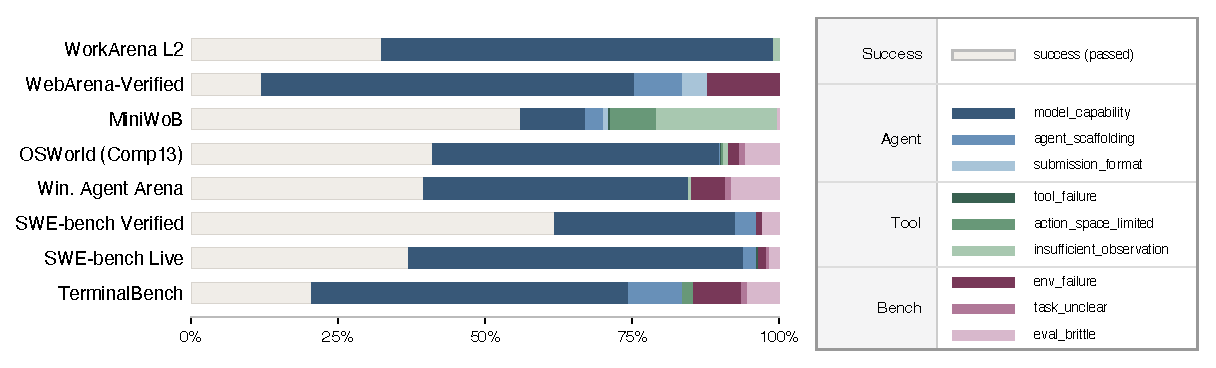
\includegraphics[width=0.92\linewidth]{figures/blame_distribution_bench}
  \caption{Blame distribution per benchmark.
  Each bar spans 100\,\% of tasks: the pale left segment is the pass rate
  (averaged over Sonnet~4.6 and GPT-5.4); the remainder is divided among
  the 9 failure-attribution categories (excluding \texttt{none}),
  scaled proportionally to the judge's blame counts.}
  \label{fig:blame-modality}
\end{figure}

Two patterns stand out. On CUA and SWE the agent-side share exceeds
80\,\%, with \texttt{model\_capability} alone accounting for roughly
four-fifths of attributions: closing this gap is the LLM-research
problem, not an evaluation one. MiniWoB is the single benchmark where
tool-side blame dominates: nearly 65\,\% of its failures hit
\texttt{action\_space\_limited} or \texttt{insufficient\_observation}
because the BrowserGym \texttt{bid} action set cannot express the
pixel-level mouse interactions that roughly 30\,\% of MiniWoB tasks
require, illustrating that tool configuration is an independent
variable. The benchmark-side share concentrates on
Windows~Agent~Arena and TerminalBench; each flagged case is a queued
issue we are iterating on
(Appendix~\ref{apdx:judge-cases}).

% --- 7.5 Qualitative judge findings ----------------------------------------
\subsection{Qualitative findings from the judge}
\label{sec:exp-qualitative}

Beyond the structured fields, the judge's free-form \emph{analysis}
acts as a curated review of the corpus. Three recurring failure
shapes show up repeatedly across our \NUMEXP{} CUBEs: capability
gaps, where the relevant evidence is in the trajectory but the agent
fails to connect it; scaffolding pathologies, typically deterministic
loops or context exhaustion that the agent cannot escape on its own;
and wrapper or evaluator bugs that only become visible once several
episodes are aggregated. Appendix~\ref{apdx:judge-cases} works
through one three-judge case per category. The benchmark-side case
(VLC \texttt{vlcrc} cluster, Table~\ref{tab:judge-case-vlc-vlcrc}) is
representative: five disjoint episodes flagged the same Python
escape-sequence trap, and a one-line \texttt{os.path.join} fix
flipped all five from 0.0 to 1.0 on resume.

% ===========================================================================
\section{Discussion}
\label{sec:discussion}
% ===========================================================================

\mypar{Wrapping a benchmark is now a small, well-scoped job.}
Under the standard, integrating a new benchmark reduces to implementing
a handful of typed classes (\texttt{Task}, \texttt{Benchmark},
\texttt{ToolConfig}) plus declarative metadata, and inheriting the
shared resource lifecycle, JSON-RPC interface, and compliance test
suite for free. In our own experience the per-benchmark wrapping cost
collapsed from weeks of bespoke harness integration to roughly a day of
focused work. We further release a \texttt{/new-cube} Claude skill that
scaffolds the wrapper, generates the metadata, and runs the compliance
checks interactively; with this tool, a benchmark author who knows their
own benchmark can produce a passing CUBE in an afternoon. We expect this
combination of a small, opinionated standard and an LLM-driven
wrapping assistant to be the dominant lever for growing the registry.

\mypar{The judge turns every run into a debugging signal.}
A recurring pattern emerged across our \NUMEXP{} CUBEs: several
independent failed episodes converge on the same root cause, and the
fix is usually a single line of wrapper or evaluator code (the VLC
cluster in \S\ref{sec:exp-qualitative} is one such case). Beyond
attributing failures to the agent, the judge therefore functions as a
continuous review of the wrappers, and of the underlying benchmarks
themselves. Several \texttt{should\_have\_been\_rewarded} verdicts in
our runs pointed at genuine ambiguity in task descriptions or
evaluator logic, artefacts that the original benchmark authors are in
a position to refine. A shared judge protocol thus turns evaluation
runs into a shared queue of triaged, evidence-backed issues for the
entire benchmark ecosystem.

\mypar{Limitations.}
Streaming actions/observations and multi-agent settings are not yet
supported and are the next protocol extensions we plan to ship;
dataset-only benchmarks remain out of scope. ``Tools held constant''
is harness-enforced rather than standard-enforced; the compliance
suite is a floor, not a correctness guarantee; faithfulness is
bounded by judge accuracy (Appendix~\ref{apdx:judge-meta}); claims
extend only to the \NUMEXP{} CUBEs evaluated.


\bibliography{references}
\bibliographystyle{plainnat}

\ifshowchecklist
\section*{NeurIPS Paper Checklist}

\begin{enumerate}

\item {\bf Claims}
    \item[] Question: Do the main claims made in the abstract and introduction accurately reflect the paper's contributions and scope?
    \item[] Answer: \answerYes{}
    \item[] Justification: \S1 enumerates four concrete contributions (standard, harness, corpus and registry, cross-benchmark experiments) and states the scope explicitly (10 CUBEs, three modalities). \S3--7 each address one contribution. No aspirational claim is left ungrounded.
    \item[] Guidelines:
    \begin{itemize}
        \item The answer \answerNA{} means that the abstract and introduction do not include the claims made in the paper.
        \item The abstract and/or introduction should clearly state the claims made, including the contributions made in the paper and important assumptions and limitations. A \answerNo{} or \answerNA{} answer to this question will not be perceived well by the reviewers.
        \item The claims made should match theoretical and experimental results, and reflect how much the results can be expected to generalize to other settings.
        \item It is fine to include aspirational goals as motivation as long as it is clear that these goals are not attained by the paper.
    \end{itemize}

\item {\bf Limitations}
    \item[] Question: Does the paper discuss the limitations of the work performed by the authors?
    \item[] Answer: \answerYes{}
    \item[] Justification: \S7 (Discussion) closes with a dedicated Limitations paragraph covering: streaming actions/observations and multi-agent settings not yet supported (flagged as the next protocol extensions on the roadmap); dataset-only benchmarks out of scope; ``tools held constant'' being harness-enforced rather than standard-enforced, so cross-benchmark comparability requires researchers to use the same \texttt{ToolConfig}; the compliance suite establishing a floor (debug tasks pass) rather than a correctness guarantee; the judge-based faithfulness signal being bounded by judge accuracy, with the meta-analysis in Appendix~\ref{apdx:judge-meta} reporting $\geq 97\%$ majority agreement but lower unanimous agreement on borderline cases; and capability claims extending only to the \NUMEXP{} CUBEs evaluated.
    \item[] Guidelines:
    \begin{itemize}
        \item The answer \answerNA{} means that the paper has no limitation while the answer \answerNo{} means that the paper has limitations, but those are not discussed in the paper.
        \item The authors are encouraged to create a separate ``Limitations'' section in their paper.
        \item The paper should point out any strong assumptions and how robust the results are to violations of these assumptions (e.g., independence assumptions, noiseless settings, model well-specification, asymptotic approximations only holding locally). The authors should reflect on how these assumptions might be violated in practice and what the implications would be.
        \item The authors should reflect on the scope of the claims made, e.g., if the approach was only tested on a few datasets or with a few runs. In general, empirical results often depend on implicit assumptions, which should be articulated.
        \item The authors should reflect on the factors that influence the performance of the approach. For example, a facial recognition algorithm may perform poorly when image resolution is low or images are taken in low lighting. Or a speech-to-text system might not be used reliably to provide closed captions for online lectures because it fails to handle technical jargon.
        \item The authors should discuss the computational efficiency of the proposed algorithms and how they scale with dataset size.
        \item If applicable, the authors should discuss possible limitations of their approach to address problems of privacy and fairness.
        \item While the authors might fear that complete honesty about limitations might be used by reviewers as grounds for rejection, a worse outcome might be that reviewers discover limitations that aren't acknowledged in the paper. The authors should use their best judgment and recognize that individual actions in favor of transparency play an important role in developing norms that preserve the integrity of the community. Reviewers will be specifically instructed to not penalize honesty concerning limitations.
    \end{itemize}

\item {\bf Theory assumptions and proofs}
    \item[] Question: For each theoretical result, does the paper provide the full set of assumptions and a complete (and correct) proof?
    \item[] Answer: \answerNA{}
    \item[] Justification: The paper presents no theoretical results. CUBE is a software standard and empirical benchmark study; all claims are engineering or empirical.
    \item[] Guidelines:
    \begin{itemize}
        \item The answer \answerNA{} means that the paper does not include theoretical results.
        \item All the theorems, formulas, and proofs in the paper should be numbered and cross-referenced.
        \item All assumptions should be clearly stated or referenced in the statement of any theorems.
        \item The proofs can either appear in the main paper or the supplemental material, but if they appear in the supplemental material, the authors are encouraged to provide a short proof sketch to provide intuition.
        \item Inversely, any informal proof provided in the core of the paper should be complemented by formal proofs provided in appendix or supplemental material.
        \item Theorems and Lemmas that the proof relies upon should be properly referenced.
    \end{itemize}

    \item {\bf Experimental result reproducibility}
    \item[] Question: Does the paper fully disclose all the information needed to reproduce the main experimental results of the paper to the extent that it affects the main claims and/or conclusions of the paper (regardless of whether the code and data are provided or not)?
    \item[] Answer: \answerYes{}
    \item[] Justification: \S6.1 specifies all evaluation details: models (4 frontier models, 2 providers), tool configuration (one per modality, held constant), agent (Genny \S4), task subsets (pre-defined splits documented per CUBE), per-step timeout, and budget cap. The harness code is available at the anonymous repository. Task subset IDs are fixed and documented.
    \item[] Guidelines:
    \begin{itemize}
        \item The answer \answerNA{} means that the paper does not include experiments.
        \item If the paper includes experiments, a \answerNo{} answer to this question will not be perceived well by the reviewers: Making the paper reproducible is important, regardless of whether the code and data are provided or not.
        \item If the contribution is a dataset and\slash or model, the authors should describe the steps taken to make their results reproducible or verifiable.
        \item Depending on the contribution, reproducibility can be accomplished in various ways. For example, if the contribution is a novel architecture, describing the architecture fully might suffice, or if the contribution is a specific model and empirical evaluation, it may be necessary to either make it possible for others to replicate the model with the same dataset, or provide access to the model. In general. releasing code and data is often one good way to accomplish this, but reproducibility can also be provided via detailed instructions for how to replicate the results, access to a hosted model (e.g., in the case of a large language model), releasing of a model checkpoint, or other means that are appropriate to the research performed.
        \item While NeurIPS does not require releasing code, the conference does require all submissions to provide some reasonable avenue for reproducibility, which may depend on the nature of the contribution. For example
        \begin{enumerate}
            \item If the contribution is primarily a new algorithm, the paper should make it clear how to reproduce that algorithm.
            \item If the contribution is primarily a new model architecture, the paper should describe the architecture clearly and fully.
            \item If the contribution is a new model (e.g., a large language model), then there should either be a way to access this model for reproducing the results or a way to reproduce the model (e.g., with an open-source dataset or instructions for how to construct the dataset).
            \item We recognize that reproducibility may be tricky in some cases, in which case authors are welcome to describe the particular way they provide for reproducibility. In the case of closed-source models, it may be that access to the model is limited in some way (e.g., to registered users), but it should be possible for other researchers to have some path to reproducing or verifying the results.
        \end{enumerate}
    \end{itemize}


\item {\bf Open access to data and code}
    \item[] Question: Does the paper provide open access to the data and code, with sufficient instructions to faithfully reproduce the main experimental results, as described in supplemental material?
    \item[] Answer: \answerYes{}
    \item[] Justification: The CUBE standard and reference harness are publicly available at the anonymous repository linked in \S3 (anonymous.4open.science, browsable without login). No new dataset is introduced; all benchmarks used are existing published resources installed at evaluation time. Installation instructions and evaluation scripts are included in the repository.
    \item[] Guidelines:
    \begin{itemize}
        \item The answer \answerNA{} means that paper does not include experiments requiring code.
        \item Please see the NeurIPS code and data submission guidelines (\url{https://neurips.cc/public/guides/CodeSubmissionPolicy}) for more details.
        \item While we encourage the release of code and data, we understand that this might not be possible, so \answerNo{} is an acceptable answer. Papers cannot be rejected simply for not including code, unless this is central to the contribution (e.g., for a new open-source benchmark).
        \item The instructions should contain the exact command and environment needed to run to reproduce the results. See the NeurIPS code and data submission guidelines (\url{https://neurips.cc/public/guides/CodeSubmissionPolicy}) for more details.
        \item The authors should provide instructions on data access and preparation, including how to access the raw data, preprocessed data, intermediate data, and generated data, etc.
        \item The authors should provide scripts to reproduce all experimental results for the new proposed method and baselines. If only a subset of experiments are reproducible, they should state which ones are omitted from the script and why.
        \item At submission time, to preserve anonymity, the authors should release anonymized versions (if applicable).
        \item Providing as much information as possible in supplemental material (appended to the paper) is recommended, but including URLs to data and code is permitted.
    \end{itemize}


\item {\bf Experimental setting/details}
    \item[] Question: Does the paper specify all the training and test details (e.g., data splits, hyperparameters, how they were chosen, type of optimizer) necessary to understand the results?
    \item[] Answer: \answerYes{}
    \item[] Justification: \S6.1 documents the model family and provider for each of the four evaluated systems, the tool configuration per modality, the agent (Genny, \S\ref{sec:harness}) and its two context-management modes, the task subsets used (full sets or pre-defined splits with rationale), the per-task step cap (150 steps), and the per-task budget cap (\$1 for small models, \$3 for large). No hyperparameters are tuned; default sampling parameters are used throughout.
    \item[] Guidelines:
    \begin{itemize}
        \item The answer \answerNA{} means that the paper does not include experiments.
        \item The experimental setting should be presented in the core of the paper to a level of detail that is necessary to appreciate the results and make sense of them.
        \item The full details can be provided either with the code, in appendix, or as supplemental material.
    \end{itemize}

\item {\bf Experiment statistical significance}
    \item[] Question: Does the paper report error bars suitably and correctly defined or other appropriate information about the statistical significance of the experiments?
    \item[] Answer: \answerYes{}
    \item[] Justification: Table~\ref{tab:passrate} reports pass rate $\pm$ 1 binomial standard error ($\sqrt{p(1-p)/n}$) for each (model, CUBE) pair, where $n$ is the effective task count (tasks $\times$ seeds where multiple seeds are used). The metric is task-binary (pass/fail), so the binomial SE is the appropriate measure of task-level variance within each evaluation subset.
    \item[] Guidelines:
    \begin{itemize}
        \item The answer \answerNA{} means that the paper does not include experiments.
        \item The authors should answer \answerYes{} if the results are accompanied by error bars, confidence intervals, or statistical significance tests, at least for the experiments that support the main claims of the paper.
        \item The factors of variability that the error bars are capturing should be clearly stated (for example, train/test split, initialization, random drawing of some parameter, or overall run with given experimental conditions).
        \item The method for calculating the error bars should be explained (closed form formula, call to a library function, bootstrap, etc.)
        \item The assumptions made should be given (e.g., Normally distributed errors).
        \item It should be clear whether the error bar is the standard deviation or the standard error of the mean.
        \item It is OK to report 1-sigma error bars, but one should state it. The authors should preferably report a 2-sigma error bar than state that they have a 96\% CI, if the hypothesis of Normality of errors is not verified.
        \item For asymmetric distributions, the authors should be careful not to show in tables or figures symmetric error bars that would yield results that are out of range (e.g., negative error rates).
        \item If error bars are reported in tables or plots, the authors should explain in the text how they were calculated and reference the corresponding figures or tables in the text.
    \end{itemize}

\item {\bf Experiments compute resources}
    \item[] Question: For each experiment, does the paper provide sufficient information on the computer resources (type of compute workers, memory, time of execution) needed to reproduce the experiments?
    \item[] Answer: \answerYes{}
    \item[] Justification: \S6.1 (\emph{Reporting}) states the per-task budget cap (\$1 for Haiku/GPT-5.4-mini, \$3 for Sonnet/GPT-5.4) and the 150-step cap; cost is computed from LiteLLM token counts multiplied by published model rates. All evaluation calls standard cloud APIs; no GPU hardware is required. Total experimental spend across the four model providers was on the order of \$20{,}000 for the full set of (model, CUBE) combinations reported in Table~\ref{tab:passrate}.
    \item[] Guidelines:
    \begin{itemize}
        \item The answer \answerNA{} means that the paper does not include experiments.
        \item The paper should indicate the type of compute workers CPU or GPU, internal cluster, or cloud provider, including relevant memory and storage.
        \item The paper should provide the amount of compute required for each of the individual experimental runs as well as estimate the total compute.
        \item The paper should disclose whether the full research project required more compute than the experiments reported in the paper (e.g., preliminary or failed experiments that didn't make it into the paper).
    \end{itemize}

\item {\bf Code of ethics}
    \item[] Question: Does the research conducted in the paper conform, in every respect, with the NeurIPS Code of Ethics \url{https://neurips.cc/public/EthicsGuidelines}?
    \item[] Answer: \answerYes{}
    \item[] Justification: The work introduces an evaluation infrastructure standard. No harmful data is collected or released, no human subjects are involved, and no privacy-sensitive information is processed. All wrapped benchmarks are used in accordance with their respective licenses.
    \item[] Guidelines:
    \begin{itemize}
        \item The answer \answerNA{} means that the authors have not reviewed the NeurIPS Code of Ethics.
        \item If the authors answer \answerNo, they should explain the special circumstances that require a deviation from the Code of Ethics.
        \item The authors should make sure to preserve anonymity (e.g., if there is a special consideration due to laws or regulations in their jurisdiction).
    \end{itemize}


\item {\bf Broader impacts}
    \item[] Question: Does the paper discuss both potential positive societal impacts and negative societal impacts of the work performed?
    \item[] Answer: \answerNA{}
    \item[] Justification: CUBE is an interoperability standard and reference harness for evaluation infrastructure; it releases no model weights, agents, training data, or generative outputs. The broader-impact surface lies with the agents being evaluated through CUBE rather than with the standard itself, and is appropriately the concern of those agent-system papers. The work makes no foundation-model or deployment claim that would warrant a societal-impact section in the paper.
    \item[] Guidelines:
    \begin{itemize}
        \item The answer \answerNA{} means that there is no societal impact of the work performed.
        \item If the authors answer \answerNA{} or \answerNo, they should explain why their work has no societal impact or why the paper does not address societal impact.
        \item Examples of negative societal impacts include potential malicious or unintended uses (e.g., disinformation, generating fake profiles, surveillance), fairness considerations (e.g., deployment of technologies that could make decisions that unfairly impact specific groups), privacy considerations, and security considerations.
        \item The conference expects that many papers will be foundational research and not tied to particular applications, let alone deployments. However, if there is a direct path to any negative applications, the authors should point it out. For example, it is legitimate to point out that an improvement in the quality of generative models could be used to generate Deepfakes for disinformation. On the other hand, it is not needed to point out that a generic algorithm for optimizing neural networks could enable people to train models that generate Deepfakes faster.
        \item The authors should consider possible harms that could arise when the technology is being used as intended and functioning correctly, harms that could arise when the technology is being used as intended but gives incorrect results, and harms following from (intentional or unintentional) misuse of the technology.
        \item If there are negative societal impacts, the authors could also discuss possible mitigation strategies (e.g., gated release of models, providing defenses in addition to attacks, mechanisms for monitoring misuse, mechanisms to monitor how a system learns from feedback over time, improving the efficiency and accessibility of ML).
    \end{itemize}

\item {\bf Safeguards}
    \item[] Question: Does the paper describe safeguards that have been put in place for responsible release of data or models that have a high risk for misuse (e.g., pre-trained language models, image generators, or scraped datasets)?
    \item[] Answer: \answerNA{}
    \item[] Justification: No model weights, generative models, or scraped datasets are released. CUBE ships only a Python interoperability standard, a reference harness, and a registry of pointers to existing benchmark packages.
    \item[] Guidelines:
    \begin{itemize}
        \item The answer \answerNA{} means that the paper poses no such risks.
        \item Released models that have a high risk for misuse or dual-use should be released with necessary safeguards to allow for controlled use of the model, for example by requiring that users adhere to usage guidelines or restrictions to access the model or implementing safety filters.
        \item Datasets that have been scraped from the Internet could pose safety risks. The authors should describe how they avoided releasing unsafe images.
        \item We recognize that providing effective safeguards is challenging, and many papers do not require this, but we encourage authors to take this into account and make a best faith effort.
    \end{itemize}

\item {\bf Licenses for existing assets}
    \item[] Question: Are the creators or original owners of assets (e.g., code, data, models), used in the paper, properly credited and are the license and terms of use explicitly mentioned and properly respected?
    \item[] Answer: \answerYes{}
    \item[] Justification: Each wrapped benchmark is cited with its original paper in \S\ref{sec:related} (\emph{Agentic benchmarks}) and listed with backend details in Appendix~\ref{apdx:bench-details}. Licenses for all upstream benchmarks are recorded in the registry YAML entry for each CUBE. The CUBE standard and reference harness are released under the Apache 2.0 license, stated in the repository.
    \item[] Guidelines:
    \begin{itemize}
        \item The answer \answerNA{} means that the paper does not use existing assets.
        \item The authors should cite the original paper that produced the code package or dataset.
        \item The authors should state which version of the asset is used and, if possible, include a URL.
        \item The name of the license (e.g., CC-BY 4.0) should be included for each asset.
        \item For scraped data from a particular source (e.g., website), the copyright and terms of service of that source should be provided.
        \item If assets are released, the license, copyright information, and terms of use in the package should be provided. For popular datasets, \url{paperswithcode.com/datasets} has curated licenses for some datasets. Their licensing guide can help determine the license of a dataset.
        \item For existing datasets that are re-packaged, both the original license and the license of the derived asset (if it has changed) should be provided.
        \item If this information is not available online, the authors are encouraged to reach out to the asset's creators.
    \end{itemize}

\item {\bf New assets}
    \item[] Question: Are new assets introduced in the paper well documented and is the documentation provided alongside the assets?
    \item[] Answer: \answerYes{}
    \item[] Justification: Three new assets are introduced and documented: (1) the CUBE standard Python package (\S3--4), with full API documentation in the anonymous repository; (2) the reference harness (\S4), documented in the same repository; (3) the CUBE registry (\S5), a GitHub-hosted file-based index with submission instructions and a compliance CI pipeline. All are available at submission time via the anonymous link in \S3.
    \item[] Guidelines:
    \begin{itemize}
        \item The answer \answerNA{} means that the paper does not release new assets.
        \item Researchers should communicate the details of the dataset\slash code\slash model as part of their submissions via structured templates. This includes details about training, license, limitations, etc.
        \item The paper should discuss whether and how consent was obtained from people whose asset is used.
        \item At submission time, remember to anonymize your assets (if applicable). You can either create an anonymized URL or include an anonymized zip file.
    \end{itemize}

\item {\bf Crowdsourcing and research with human subjects}
    \item[] Question: For crowdsourcing experiments and research with human subjects, does the paper include the full text of instructions given to participants and screenshots, if applicable, as well as details about compensation (if any)?
    \item[] Answer: \answerNA{}
    \item[] Justification: No crowdsourcing or research with human subjects is involved. All evaluation uses automated, environment-based judges; no human annotators or participants are used.
    \item[] Guidelines:
    \begin{itemize}
        \item The answer \answerNA{} means that the paper does not involve crowdsourcing nor research with human subjects.
        \item Including this information in the supplemental material is fine, but if the main contribution of the paper involves human subjects, then as much detail as possible should be included in the main paper.
        \item According to the NeurIPS Code of Ethics, workers involved in data collection, curation, or other labor should be paid at least the minimum wage in the country of the data collector.
    \end{itemize}

\item {\bf Institutional review board (IRB) approvals or equivalent for research with human subjects}
    \item[] Question: Does the paper describe potential risks incurred by study participants, whether such risks were disclosed to the subjects, and whether Institutional Review Board (IRB) approvals (or an equivalent approval/review based on the requirements of your country or institution) were obtained?
    \item[] Answer: \answerNA{}
    \item[] Justification: No human subjects are involved; IRB approval is not applicable.
    \item[] Guidelines:
    \begin{itemize}
        \item The answer \answerNA{} means that the paper does not involve crowdsourcing nor research with human subjects.
        \item Depending on the country in which research is conducted, IRB approval (or equivalent) may be required for any human subjects research. If you obtained IRB approval, you should clearly state this in the paper.
        \item We recognize that the procedures for this may vary significantly between institutions and locations, and we expect authors to adhere to the NeurIPS Code of Ethics and the guidelines for their institution.
        \item For initial submissions, do not include any information that would break anonymity (if applicable), such as the institution conducting the review.
    \end{itemize}

\item {\bf Declaration of LLM usage}
    \item[] Question: Does the paper describe the usage of LLMs if it is an important, original, or non-standard component of the core methods in this research? Note that if the LLM is used only for writing, editing, or formatting purposes and does \emph{not} impact the core methodology, scientific rigor, or originality of the research, declaration is not required.
    \item[] Answer: \answerYes{}
    \item[] Justification: LLMs are a core methodological component in three roles: (1) the evaluated systems, where the paper measures frontier LLM-based agents across the corpus; (2) the trajectory judge (\S\ref{sec:judge}), where a Claude Code agent reads recorded episodes and produces structured failure attributions; (3) the \texttt{/new-cube} and \texttt{/review-cube} authoring skills (\S\ref{sec:standard}), where Claude Code agents generate and audit CUBE boilerplate. All three roles are described in the paper.
    \item[] Guidelines:
    \begin{itemize}
        \item The answer \answerNA{} means that the core method development in this research does not involve LLMs as any important, original, or non-standard components.
        \item Please refer to our LLM policy in the NeurIPS handbook for what should or should not be described.
    \end{itemize}

\end{enumerate}

\fi

% ===========================================================================
% APPENDICES (after \bibliography in NeurIPS template)
% ===========================================================================
% A. JSON-RPC interface details (the protocol material the main text deliberately does not include).
% B. Per-benchmark task count, license, infra requirements.
% C. Tool configuration details and ablation tables that did not fit.
% D. Composite construction reproducibility: the exact baseline run seeds, tier thresholds, sampled task IDs.

\newpage

\appendix

\begin{center}
  {\LARGE\textbf{Appendix}}
\end{center}
\vspace{1em}

\section{JSON-RPC interface details}
\label{apdx:json-rpc-protocol}

The standard auto-generates a JSON-RPC~2.0 server from any \texttt{Benchmark} subclass.
The server exposes two endpoints whose names and payload shape match MCP's \texttt{tools/list} and \texttt{tools/call}, so any MCP-compatible client (LLM tool-call loop, IDE plugin, evaluation harness) can drive a CUBE task without an adapter layer.

\mypar{Endpoint: \texttt{tools/list}.}
Returns the action schema derived from the task's default tool: one entry per \texttt{@tool\_action}-decorated method, with name, description, and JSON Schema for the arguments. The schema is generated at task construction time and is static for the lifetime of the episode.

\mypar{Endpoint: \texttt{tools/call}.}
Accepts \texttt{\{name, arguments\}} and routes to \texttt{task.step(Action(name, arguments))}, returning the serialized \texttt{EnvironmentOutput} (observation, done flag, reward if terminal, info dict). A call after \texttt{done=True} raises a protocol error; the client must call \texttt{tools/list} on a fresh session to start a new episode.

\mypar{Server lifecycle.}
\texttt{Benchmark.\_setup()} starts the server (one per benchmark, shared across tasks); \texttt{Benchmark.close()} tears it down. Individual tasks register and deregister their endpoints on \texttt{reset()} and episode end. The server address is published in \texttt{RuntimeContext} so remote workers can connect without further coordination.

% \newpage

\section{Per-benchmark task count, license, infra requirements}
\label{apdx:bench-details}

\begin{table}[h]
\centering
\caption{The CUBE registry at submission.}
\label{tab:cubes}
\footnotesize
\setlength{\tabcolsep}{5pt}
\renewcommand{\arraystretch}{1.05}
\begin{tabular}{llrl}
\toprule
\textbf{CUBE} & \textbf{Modality} & \textbf{\# Tasks} & \textbf{Backend} \\
\midrule
WorkArena            & Web      & 333    & Live enterprise web app \\
WebArena-Verified    & Web      & 812    & Shared 6-service Docker stack \\
MiniWoB              & Web      & 125    & Local browser \\
BrowseComp          & Web      & 1{,}266 & Browser \\
OSWorld              & CUA      & 368    & Ubuntu 22.04 VM \\
Windows Agent Arena  & CUA      & 154    & Windows 11 VM \\
SWE-bench Verified   & SWE      & 500    & Per-task Docker \\
SWE-bench Live       & SWE      & 1{,}895 & Per-task Docker \\
Terminal-Bench        & Terminal & 89     & Per-task Docker \\
DRBench              & Research & 100    & Per-task Docker (Nextcloud, Mattermost, IMAP) \\
\midrule
\textbf{Total}       &          & \textbf{5{,}642} & \\
\bottomrule
\end{tabular}
\end{table}

\section{Judge output schema and blame taxonomy}
\label{apdx:judge-schema}

\mypar{Output schema.}
Each \texttt{JudgeOutput} carries five fields: an \emph{outcome}
(\texttt{success}, \texttt{success\_lucky}, \texttt{almost},
\texttt{failure}, \texttt{should\_have\_been\_rewarded}); a \emph{primary
blame} from the closed taxonomy plus optional \emph{secondary blames};
\emph{evidence}, the step-indexed verbatim quotes; a \emph{hypothesis} of
what would fix the failure class; and 0--5 confidence scores on both
blame and hypothesis. A free-form \emph{analysis} field placed first acts
as a reasoning scratchpad before the structured fields are committed.

\mypar{Blame taxonomy.}
Ten benchmark-agnostic categories grouped into three buckets.
\textbf{Agent-side}: \texttt{model\_capability} (the LLM lacked the
reasoning, knowledge, or planning to solve the task);
\texttt{agent\_scaffolding} (the agent loop, prompt, or context
management caused the failure); \texttt{submission\_format} (the agent
reached a solution but failed to submit it through the registered
channel). \textbf{Tool-side}: \texttt{tool\_failure} (a tool wrapper
raised or returned an unexpected error); \texttt{action\_space\_limited}
(no available action could express the correct solution);
\texttt{insufficient\_observation} (the rendered observation hid
information the agent needed). \textbf{Benchmark-side}:
\texttt{env\_failure} (infrastructure crash outside the agent's and
tool's control); \texttt{task\_unclear} (the task description is
ambiguous or contradictory); \texttt{eval\_brittle} (the evaluator
rejected an acceptable solution). A residual \texttt{none} category is
assigned on clean success or when evidence is insufficient for any
attribution.

\section{Drift sources in dynamic-agent benchmarks}
\label{apdx:reproducibility}

Five sources of drift recur across the corpus and motivate the
reliability framing of Appendix~\ref{apdx:reproducibility}.

\mypar{Scaffolding sensitivity.}
Pass rate depends heavily on the agent loop, the tool wrappers, the
prompt boilerplate, and the exact context-management strategy. Two
scaffolds calling the same model can differ by tens of points on the
same benchmark; cross-benchmark comparisons that mix scaffolds are not
measuring the model.

\mypar{Prompt tailoring.}
Many published numbers use a prompt or chain-of-thought structure tuned
for a specific benchmark, sometimes with in-context examples drawn from
its training split. The reported number is then a joint property of the
model and the prompt-engineering effort, not of the model in a
generalist setting.

\mypar{Model version drift.}
Frontier APIs are continuously retrained and behaviour-tuned. A model
identifier (\texttt{claude-sonnet-4-6}, \texttt{gpt-5.4}) names a moving
target whose behaviour at the time of a published number may not be
reproducible months later.

\mypar{Closed-source scaffolds.}
Strong leaderboard numbers are sometimes reported by labs whose
scaffold, tool stack, and prompt are not released, in contexts where
headline numbers carry commercial weight. These results are not
reproducible by construction.

\mypar{Live-component drift.}
Several benchmarks in the corpus depend on live external services or
system state that change without notice: WorkArena targets a live
enterprise web application; OSWorld and Windows Agent Arena depend on
OS revisions; underlying browser-automation libraries
(\texttt{playwright}, \texttt{pyautogui}) ship breaking updates between
minor versions. Two runs weeks apart against the same task set can
produce different ground-truth pass rates.

\section{Judge meta-analysis}
\label{apdx:judge-meta}

For every episode that received three independent judge invocations we
measure \emph{primary-blame agreement} (do all three judges choose the
same blame category?) and \emph{outcome agreement} (do all three agree on
pass / almost / fail?).
Tables~\ref{tab:agree-blame} and~\ref{tab:agree-outcome} report the counts
and rates for the two benchmarks where triple-judge runs were completed:
SWE-bench~Verified (Sonnet~4.6, $n{=}162$; GPT-5.4, $n{=}204$) and
SWE-bench~Live (Sonnet~4.6, $n{=}83$).

\begin{table}[h]
\centering
\caption{Primary-blame agreement across three independent judges.
  \emph{3/3}: all three choose the same category.
  \emph{2/3}: a two-judge majority.
  \emph{All differ}: no two judges agree.
  ${\geq}2/3$ subsumes both 3/3 and 2/3 rows.}
\label{tab:agree-blame}
\small
\setlength{\tabcolsep}{6pt}
\renewcommand{\arraystretch}{1.15}
\begin{tabular}{llrrrrrr}
\toprule
Benchmark & Model & $n$ & 3/3 & 2/3 & All differ & 3/3\,\% & ${\geq}2/3$\,\% \\
\midrule
SWE-bench Verified & Sonnet~4.6 & 162 & 117 & 40 & 5 & 72.2 & 96.9 \\
SWE-bench Verified & GPT-5.4    & 204 & 173 & 27 & 4 & 84.8 & 98.0 \\
SWE-bench Live     & Sonnet~4.6 &  83 &  64 & 19 & 0 & 77.1 & 100.0 \\
\bottomrule
\end{tabular}
\end{table}

\begin{table}[h]
\centering
\caption{Outcome agreement (pass / almost / fail) across three independent judges.
  Column definitions identical to Table~\ref{tab:agree-blame}.}
\label{tab:agree-outcome}
\small
\setlength{\tabcolsep}{6pt}
\renewcommand{\arraystretch}{1.15}
\begin{tabular}{llrrrrrr}
\toprule
Benchmark & Model & $n$ & 3/3 & 2/3 & All differ & 3/3\,\% & ${\geq}2/3$\,\% \\
\midrule
SWE-bench Verified & Sonnet~4.6 & 162 & 114 & 46 & 2 & 70.4 & 98.8 \\
SWE-bench Verified & GPT-5.4    & 204 & 126 & 77 & 1 & 61.8 & 99.5 \\
SWE-bench Live     & Sonnet~4.6 &  83 &  77 &  6 & 0 & 92.8 & 100.0 \\
\bottomrule
\end{tabular}
\end{table}

\paragraph{Takeaways.}
Majority (${\geq}2/3$) agreement is \textbf{97–100\,\%} across every
condition for both blame and outcome, meaning the modal vote is almost
always stable and reliable as a signal.
Full unanimous agreement is somewhat lower — \textbf{62–85\,\%} for blame
and \textbf{62–93\,\%} for outcome — which is expected: the taxonomy
contains adjacent categories (\emph{model\_capability} vs.\
\emph{agent\_scaffolding}) that can legitimately both apply to the same
failure, and the outcome three-way split (pass / almost / fail) places
hard boundaries on a continuous quality gradient.

The hardest condition is SWE-bench~Verified outcome for GPT-5.4, where
unanimous agreement falls to 61.8\,\%.
We attribute this to the high overall pass rate on that benchmark
(${\approx}58\,\%$): many GPT-5.4 episodes produce partial fixes that
sit ambiguously between \emph{almost} and \emph{fail}, a genuinely
difficult judgement call even for human annotators.
Notably, the \emph{all-differ} rate (complete three-way disagreement)
stays below 2.5\,\% in every condition, confirming that true confusion is
rare and that majority voting is a robust aggregation strategy.

% \newpage

\section{Judge case studies}
\label{apdx:judge-cases}

Table~\ref{tab:judge-case-astropy} shows a representative case in which all
three judges unanimously converge, illustrating both the evidence-grounding
mechanism and the blame attribution in practice.  The episode is drawn from
the SWE-bench~Verified run (\S\ref{sec:experiments}); the judge had access to
the full step-indexed trajectory and the privileged evaluation output.

\begin{table*}[h]
\centering
\caption{%
  Three independent judge outputs for episode
  \texttt{astropy\_\_astropy-14365} (SWE-bench~Verified, outcome
  \emph{almost}).  All three judges unanimously agree on primary blame and
  intervention; high-confidence evidence quotes pinpoint the unfixed
  downstream \texttt{if\,v\,==\,"NO":} comparison that the agent read but
  failed to connect to its own regex fix.
  Evidence quotes are verbatim from the judge output; long code blocks are
  truncated at [\ldots] to fit the column.
}
\label{tab:judge-case-astropy}
\scriptsize
\setlength{\tabcolsep}{4pt}
\renewcommand{\arraystretch}{1.4}
\definecolor{rowgray}{HTML}{F2F2F2}
\begin{tabularx}{\linewidth}{@{} >{\bfseries\RaggedRight}p{2.0cm}
                                  >{\RaggedRight\arraybackslash}X
                                  >{\RaggedRight\arraybackslash}X
                                  >{\RaggedRight\arraybackslash}X @{}}
\toprule
Field & Judge 1 & Judge 2 & Judge 3 \\
\midrule
\rowcolor{rowgray}
Outcome & \emph{almost} & \emph{almost} & \emph{almost} \\
Primary blame
  & \texttt{model\_capability} (conf.\,4/5)
  & \texttt{model\_capability} (conf.\,3/5)
  & \texttt{model\_capability} (conf.\,4/5) \\
\rowcolor{rowgray}
Secondary & \texttt{agent\_scaffolding} & -- & \texttt{agent\_scaffolding} \\
Summary
  & Added \texttt{re.IGNORECASE} to QDP command regex but missed downstream
    \texttt{if\,v\,==\,"NO":} null-marker check; verified only syntax
    compilation, never ran the test suite.
  & Fix incomplete: \texttt{re.IGNORECASE} applied to command recognition;
    null-value sentinel \texttt{"NO"} still compared case-sensitively;
    crashes on lowercase \texttt{"no"} with \texttt{ValueError}.
  & Regex fix correct for command recognition; identical case-sensitivity
    bug in data-value processing loop not connected; \texttt{final\_step}
    called without running any tests. \\
\rowcolor{rowgray}
Key evidence
  & \textit{step~8} (verified):\newline
    {\ttfamily for v in line.split(delimiter):\newline
    \phantom{xxxx}if v == "NO":\newline
    \phantom{xxxxxxxx}...\newline
    \phantom{xxxx}else: [...]}%
    \medskip\newline
    \textit{step~16} (verified):\newline
    {\ttfamily ValueError: could not convert string to float: 'no'}
  & \textit{step~56} (verified, match\,0.88):\newline
    {\ttfamily ValueError: could not convert string to float: 'no'\newline
    astropy/io/ascii/qdp.py:317: ValueError}
  & \textit{step~8} (verified):\newline
    {\ttfamily for v in line.split(delimiter):\newline
    \phantom{xxxx}if v == "NO":\newline
    \phantom{xxxxxxxx}...\newline
    \phantom{xxxx}else: [...]}%
    \medskip\newline
    \textit{step~15} (verified):\newline
    {\ttfamily ACTION final\_step:\newline
    \{\}} \\
Hypothesis
  & Change \texttt{"NO"} to \texttt{v.upper()\,==\,"NO"} throughout;
    mandate \texttt{pytest} run on the failing test before submit.
  & Run the actual failing test before submitting; would reveal the
    secondary failure immediately.
  & Add mandatory post-fix validation step (run failing reproduction case)
    to the agent workflow. \\
\rowcolor{rowgray}
Intervention
  & \texttt{prompt\_change} (conf.\,3/5)
  & \texttt{prompt\_change} (conf.\,3/5)
  & \texttt{prompt\_change} (conf.\,4/5) \\
\bottomrule
\end{tabularx}
\end{table*}

\begin{table*}[t]
\centering
\caption{%
  Three independent judge outputs for episode
  \texttt{conan-io\_\_conan-18028} (SWE-bench~Live, outcome \emph{failure}).
  The agent located \texttt{graph\_builder.py} and the \texttt{skip\_test}
  check at step~82, then immediately fell into a deterministic loop,
  re-issuing the same \texttt{grep} command 53 consecutive times and hitting
  \texttt{MAX\_STEPS\_REACHED} without writing a single line of code.
  All three judges agree on \texttt{scaffold\_change} as the intervention;
  two of three assign primary blame to \texttt{agent\_scaffolding}.
  Evidence quotes are verbatim from the judge output; long action strings
  are truncated at [\ldots] to fit the column.
}
\label{tab:judge-case-conan-18028}
\scriptsize
\setlength{\tabcolsep}{4pt}
\renewcommand{\arraystretch}{1.4}
\definecolor{rowgray}{HTML}{F2F2F2}
\begin{tabularx}{\linewidth}{@{} >{\bfseries\RaggedRight}p{2.0cm}
                                  >{\RaggedRight\arraybackslash}X
                                  >{\RaggedRight\arraybackslash}X
                                  >{\RaggedRight\arraybackslash}X @{}}
\toprule
Field & Judge 1 & Judge 2 & Judge 3 \\
\midrule
\rowcolor{rowgray}
Outcome & \emph{failure} & \emph{failure} & \emph{failure} \\
Primary blame
  & \texttt{agent\_scaffolding} (conf.\,5/5)
  & \texttt{model\_capability} (conf.\,4/5)
  & \texttt{agent\_scaffolding} (conf.\,4/5) \\
\rowcolor{rowgray}
Secondary & \texttt{model\_capability} & \texttt{agent\_scaffolding} & \texttt{model\_capability} \\
Summary
  & Spent all 150 steps in read-only exploration, running identical
    \texttt{grep} commands dozens of times without writing a single code
    edit or calling \texttt{final\_step}.
  & Spent all 150 steps in \texttt{grep}/\texttt{cat} exploration; from
    step~80 fell into a tight loop re-running the same \texttt{grep} with
    identical output each time.
  & Located \texttt{tools.graph:skip\_test} in \texttt{graph\_builder.py}
    at step~81, then immediately fell into a deterministic loop: same
    \texttt{grep} command 53 consecutive times, 0 code edits,
    \texttt{MAX\_STEPS\_REACHED}. \\
\rowcolor{rowgray}
Key evidence
  & \textit{steps~99, 101, 103} (verified, match\,0.86):\newline
    {\ttfamily ACTION bash: \{...\,grep -rn\newline
    \phantom{xx}"skip\_test\textbar{}tools.graph:skip\_test"\newline
    \phantom{xx}.../graph\_builder.py\}}\medskip\newline
    \textit{steps~295, 297, 299} (verified, match\,0.90):\newline
    {\ttfamily ACTION bash: \{...\,grep -rn\newline
    \phantom{xx}"node\.test\textbackslash b" conans/ conan/\newline
    \phantom{xx}--include="*.py"\,|\,grep -v "test/"\}}
  & \textit{step~81} (verified, match\,0.86):\newline
    {\ttfamily ACTION bash: \{...\,grep -rn\newline
    \phantom{xx}"skip\_test\textbar{}tools.graph:skip\_test"\newline
    \phantom{xx}.../graph\_builder.py\}}\medskip\newline
    \textit{step~121} (verified, match\,0.86):\newline
    {\ttfamily ACTION bash: \{...\,grep -rn\newline
    \phantom{xx}"skip\_test\textbar{}tools.graph:skip\_test"\newline
    \phantom{xx}.../graph\_builder.py\}}
  & \textit{step~82} (verified):\newline
    {\ttfamily 216:\phantom{x}skip\_test = node.conanfile.conf\newline
    \phantom{xxxxxx}.get("tools.graph:skip\_test",...)\newline
    222:\phantom{x}if skip\_test and require.test:}\medskip\newline
    \textit{step~83\,\textrightarrow\,151} (loop begins):\newline
    {\ttfamily ACTION bash: \{...\,grep -rn\newline
    \phantom{xx}"skip\_test\textbar{}tools.graph:skip\_test"\newline
    \phantom{xx}.../graph\_builder.py\}}\medskip\newline
    \textit{metadata} (step~0):\newline
    {\ttfamily "status": "MAX\_STEPS\_REACHED",\newline
    "prompt\_tokens": 6430181,\newline
    "cached\_tokens": 6267737} \\
Hypothesis
  & Adding loop detection (block on $N$ consecutive identical tool calls)
    and context compaction at a reasonable threshold would prevent this
    class of failure.
  & A scaffold with loop detection would have interrupted the cycle and
    forced a different action; the agent had located the relevant code but
    lacked the push to synthesize an edit.
  & Full history, temperature~0, and no compaction create a deterministic
    feedback loop once repetition starts; aborting after $K$ consecutive
    identical actions would break the cycle. \\
\rowcolor{rowgray}
Intervention
  & \texttt{scaffold\_change} (conf.\,5/5)
  & \texttt{scaffold\_change} (conf.\,3/5)
  & \texttt{scaffold\_change} (conf.\,5/5) \\
\bottomrule
\end{tabularx}
\end{table*}


% Case study: VLC vlcrc path corruption (Sonnet × T1, WAA campaign)
% 5 independent episodes, 5 independent judge analyses, 1 root cause,
% 1 one-line fix, 5/5 flipped 0.0 -> 1.0 on resume.

\begin{table*}[t]
\centering
\caption{%
  Three independent judges on three WAA episodes
  (\texttt{ep87}, \texttt{ep88}, \texttt{ep151}; all VLC-domain, all scored 0.0),
  working on disjoint trajectories with no shared context.
  All three converge on the same eval-side root cause: the \texttt{vlcrc}
  path string passed to \texttt{execute\_python\_command} is re-parsed as
  Python source, silently collapsing \texttt{\textbackslash{}v} to
  U+000B (vertical tab) and corrupting the path before \texttt{get\_file()}
  sees it.  A one-line \texttt{os.path.join} fix on the VM side flipped
  all five affected episodes from 0.0 to 1.0 on a single resumed run.
}
\label{tab:judge-case-vlc-vlcrc}
\scriptsize
\setlength{\tabcolsep}{4pt}
\renewcommand{\arraystretch}{1.4}
\definecolor{rowgray}{HTML}{F2F2F2}
\begin{tabularx}{\linewidth}{@{} >{\bfseries\RaggedRight}p{2.0cm}
                                  >{\RaggedRight\arraybackslash}X
                                  >{\RaggedRight\arraybackslash}X
                                  >{\RaggedRight\arraybackslash}X @{}}
\toprule
Field & Judge / ep87 & Judge / ep88 & Judge / ep151 \\
\midrule
\rowcolor{rowgray}
Outcome
  & \emph{should\_have\_been\_rewarded}
  & \emph{should\_have\_been\_rewarded}
  & \emph{should\_have\_been\_rewarded} \\
Primary blame
  & \texttt{eval\_brittle} (conf.\,3/5)
  & \texttt{eval\_brittle} (conf.\,3/5)
  & \texttt{tool\_failure} (conf.\,2/5) \\
\rowcolor{rowgray}
Task
  & Set VLC recording folder to Downloads
  & Set VLC recording folder to Desktop
  & Disable ``Resize interface to video size'' in VLC \\
Summary
  & Agent completed navigation (Preferences\,$\to$\,[\ldots]\,$\to$\,Downloads\,$\to$\,Save).
    Evaluator's \texttt{get\_vlc\_config} path literal re-parsed as Python;
    \texttt{\textbackslash v}\,$\to$\,U+000B corrupted \texttt{\textbackslash vlcrc}
    to \texttt{\textbackslash u000blcrc}; \texttt{get\_file} 500, false \texttt{FileNotFoundError}.
  & Agent navigated Preferences and set Desktop as recording folder and saved.
    Evaluator's \texttt{get\_vlc\_config} path literal re-parsed as Python;
    \texttt{\textbackslash v}\,$\to$\,U+000B corrupted \texttt{\textbackslash vlcrc}
    to \texttt{\textbackslash u000blcrc}; \texttt{get\_file} 500, score 0.0.
  & Agent navigated Preferences and unchecked `Resize interface to video size.'
    Evaluator's \texttt{get\_vlc\_config} path literal re-parsed as Python;
    \texttt{\textbackslash v}\,$\to$\,U+000B corrupted \texttt{\textbackslash vlcrc}
    to \texttt{\textbackslash u000blcrc}; \texttt{get\_file} 500, false \texttt{FileNotFoundError}. \\
\rowcolor{rowgray}
Key evidence
  & \textit{step~9} (verified):\newline
    {\ttfamily [ERROR] get\_file() ---\newline
    \phantom{xx}C:\textbackslash Users\textbackslash Docker\textbackslash AppData\textbackslash\newline
    \phantom{xx}Roaming\textbackslash u000blc\textbackslash u000blcrc}
  & \textit{step~9} (verified):\newline
    {\ttfamily [ERROR] get\_file() ---\newline
    \phantom{xx}C:\textbackslash Users\textbackslash Docker\textbackslash AppData\textbackslash\newline
    \phantom{xx}Roaming\textbackslash u000blc\textbackslash u000blcrc}
  & \textit{step~8} (verified):\newline
    {\ttfamily ACTION run\_pyautogui:\newline
    \phantom{xx}\{"code": "pyautogui.click(\newline
    \phantom{xx}784, 689) \# Save"\}}\medskip\newline
    \textit{step~9} (verified):\newline
    {\ttfamily [ERROR] get\_file() ---\newline
    \phantom{xx}Roaming\textbackslash u000blc\textbackslash u000blcrc} \\
Hypothesis
  & Path literal \texttt{\textbackslash vlcrc} in \texttt{execute\_python\_command}
    re-parsed as Python source; \texttt{\textbackslash v}\,$\to$\,U+000B.
    Replace with \texttt{os.path.join} to eliminate escape-sequence literals.
  & Classic escape-sequence trap on the Python round-trip.
    Build path from \texttt{os.path.join} components
    so no \texttt{\textbackslash v} literal survives re-parse.
  & \texttt{get\_vlc\_config} sends a Python expression to the VM;
    \texttt{\textbackslash v} in \texttt{\textbackslash vlcrc} collapses to U+000B silently.
    Switch to \texttt{os.path.join('\textasciitilde',\,\ldots,\,'vlcrc')}. \\
\rowcolor{rowgray}
Intervention
  & \texttt{eval\_fix} (conf.\,4/5)
  & \texttt{eval\_fix} (conf.\,4/5)
  & \texttt{eval\_fix} (conf.\,3/5) \\
Post-fix outcome
  & \textbf{0.0\,$\to$\,1.0} on resume (\texttt{is\_vlc\_recordings\_folder} score 1.0)
  & \textbf{0.0\,$\to$\,1.0} on resume (\texttt{is\_vlc\_recordings\_folder} score 1.0)
  & \textbf{0.0\,$\to$\,1.0} on resume (\texttt{is\_vlc\_resize\_video\_disabled} score 1.0) \\
\bottomrule
\end{tabularx}
\end{table*}

% --- Suggested narrative paragraph ---
%
% Across 65 failed Sonnet T1 episodes, the judge attributed 20 (33\%) to
% \texttt{eval\_brittle}. Five of those --- \texttt{ep30}, \texttt{ep87},
% \texttt{ep88}, \texttt{ep135}, \texttt{ep151} --- share an identical root
% cause that no individual judge run could have established alone: a Python
% escape-sequence trap in the WAA cube's \texttt{get\_vlc\_config} helper.
% The judge's per-episode analyses converge on the same hypothesis
% (Table~\ref{tab:judge-case-vlc-vlcrc}); a one-line \texttt{os.path.join}
% change on the VM side flipped all five episodes from 0.0 to 1.0 in a
% single resumed run, raising the Sonnet T1 pass rate by 3.3 pp and
% confirming the bug was eval-side rather than agent-side. This pattern ---
% independent judgments converging on a shared, machine-verifiable root
% cause --- is what makes blame attribution actionable at scale.

% Case 3A: GPT-5.4 run — split verdict (model used wrong clipboard method)
\begin{table*}[t]
\centering
\caption{%
  Three independent judge outputs for episode \texttt{716a6079\_ep235}
  (\textbf{GPT-5.4 run}, OSWorld, outcome consensus: \emph{failure}).
  Task: find \texttt{secret.docx} on the VM and copy its full path to the
  clipboard. File is at \texttt{/home/user/Data3/List3/secret.docx}.
  The three judges \emph{disagree} on root cause: Judge~1 blames the model
  (agent used \texttt{Ctrl+L} in Nautilus, which copies the containing
  \emph{directory} path, not the full file path, and rates the outcome
  \emph{almost} --- a near-miss sub-category of failure); Judges~2--3 blame
  infrastructure (\texttt{xsel} is not installed on the VM, so the evaluator
  \texttt{is\_in\_vm\_clickboard} always reads an empty clipboard regardless
  of agent behavior). This split illustrates a compound failure: a
  model-capability weakness \emph{and} a broken infrastructure-level
  evaluator co-occur, making the true verdict ambiguous.
  Compare with Table~\ref{tab:judge-case-clipboard-xsel-sonnet} (Sonnet run,
  same task): Sonnet used \texttt{xclip} correctly and received a unanimous
  \emph{should\_have\_been\_rewarded}.
}
\label{tab:judge-case-clipboard-xsel-gpt4}
\scriptsize
\setlength{\tabcolsep}{4pt}
\renewcommand{\arraystretch}{1.4}
\definecolor{rowgray}{HTML}{F2F2F2}
\begin{tabularx}{\linewidth}{@{} >{\bfseries\RaggedRight}p{2.2cm}
                                  >{\RaggedRight\arraybackslash}X
                                  >{\RaggedRight\arraybackslash}X
                                  >{\RaggedRight\arraybackslash}X @{}}
\toprule
Field & Judge 1 & Judge 2 & Judge 3 \\
\midrule
\rowcolor{rowgray}
Outcome & \emph{almost} & \emph{failure} & \emph{failure} \\
Primary blame
  & \texttt{model\_capability} (conf.\,3/5)
  & \texttt{eval\_brittle} (conf.\,4/5)
  & \texttt{env\_failure} (conf.\,4/5) \\
\rowcolor{rowgray}
Secondary & \texttt{action\_space\_limited} & \texttt{model\_capability} & \texttt{model\_capability} \\
Summary
  & Agent found the correct file but used \texttt{Ctrl+L}+\texttt{Ctrl+C}
    in Nautilus, which copies the \emph{directory} path, not the full
    file path. Clipboard contained \texttt{/home/user/Data3/List3}
    instead of \texttt{\ldots/secret.docx}.
  & \texttt{xsel} is not installed on the VM (\texttt{returncode~127}),
    making clipboard scoring impossible for any agent. Separately,
    agent's \texttt{Ctrl+L}+\texttt{Ctrl+C} would have produced the
    directory path, not the file path.
  & VM missing \texttt{xsel} binary that \texttt{is\_in\_vm\_clickboard}
    relies on; evaluator always returns empty output, making reward=0
    inevitable regardless of agent behavior. \\
\rowcolor{rowgray}
Key evidence
  & \textit{step~29} (verified, match\,0.94):\newline
    {\ttfamily ACTION hotkey: \{"keys": "ctrl+l"\}}\medskip\newline
    \textit{step~31} (verified, match\,0.94):\newline
    {\ttfamily ACTION hotkey: \{"keys": "ctrl+c"\}}\medskip\newline
    \textit{task config}:\newline
    {\ttfamily "expected": "/home/user/Data3/\newline List3/secret.docx"}
  & \textit{evaluator log} (match\,0.34):\newline
    {\ttfamily \{'error':\newline '/bin/sh: 1: xsel: not found\textbackslash n',\newline
    'output': '', 'returncode': 127\}}\medskip\newline
    \textit{evaluator log} (match\,0.52):\newline
    {\ttfamily reward=0.000000,\newline evaluator=is\_in\_vm\_clickboard}\medskip\newline
    \textit{step~29} (verified, match\,0.94):\newline
    {\ttfamily ACTION hotkey: \{"keys": "ctrl+l"\}}
  & \textit{evaluator log}:\newline
    {\ttfamily \{'error': '/bin/sh: 1:\newline xsel: not found\textbackslash n',\newline
    'returncode': 127, 'output': ''\}}\medskip\newline
    \textit{evaluator}:\newline
    {\ttfamily is\_in\_vm\_clickboard} depends on\newline \texttt{xsel --clipboard --output} \\
Hypothesis
  & Instruct agent to use file Properties dialog or right-click
    `Copy Location' to obtain full file path; \texttt{Ctrl+L} in
    Nautilus yields only the directory.
  & Install \texttt{xsel} on VM base image, or update evaluator to
    fall back to \texttt{xclip -o -selection clipboard}; also fix
    agent clipboard strategy.
  & VM image (cube-ubuntu-22-04 v1.0.0) does not include \texttt{xsel};
    install \texttt{xsel} or switch evaluator to \texttt{xclip -o} or
    \texttt{wl-paste} to fix all clipboard-check tasks. \\
\rowcolor{rowgray}
Intervention
  & \texttt{prompt\_change} (conf.\,3/5)
  & \texttt{eval\_fix} (conf.\,5/5)
  & \texttt{infra\_fix} (conf.\,5/5) \\
\bottomrule
\end{tabularx}
\end{table*}

% Case 3B: Sonnet run — unanimous should_have_been_rewarded
\begin{table*}[t]
\centering
\caption{%
  Three independent judge outputs for episode \texttt{716a6079\_ep235}
  (\textbf{Sonnet run}, OSWorld, outcome consensus: \emph{should\_have\_been\_rewarded}).
  \emph{Same task as Table~\ref{tab:judge-case-clipboard-xsel-gpt4}.}
  Unlike GPT-5.4 (which used \texttt{Ctrl+L} in Nautilus and copied only
  the directory path), the Sonnet agent correctly used
  \texttt{xclip -selection clipboard} in a terminal to copy the full file
  path \texttt{/home/user/Data3/List3/secret.docx}.
  All three judges agree: the correct agent action was irrelevant because
  the evaluator's clipboard-reading command (\texttt{xsel --clipboard
  --output}) is not installed on the VM, so the clipboard always reads
  as empty.
  This cross-model pair is direct evidence that the same broken evaluator
  can produce a \emph{model-capability failure} verdict for a weaker agent
  and a \emph{should\_have\_been\_rewarded} verdict for a stronger one ---
  masking genuine capability differences behind infrastructure noise.
}
\label{tab:judge-case-clipboard-xsel-sonnet}
\scriptsize
\setlength{\tabcolsep}{4pt}
\renewcommand{\arraystretch}{1.4}
\definecolor{rowgray}{HTML}{F2F2F2}
\begin{tabularx}{\linewidth}{@{} >{\bfseries\RaggedRight}p{2.2cm}
                                  >{\RaggedRight\arraybackslash}X
                                  >{\RaggedRight\arraybackslash}X
                                  >{\RaggedRight\arraybackslash}X @{}}
\toprule
Field & Judge 1 & Judge 2 & Judge 3 \\
\midrule
\rowcolor{rowgray}
Outcome & \emph{should\_have\_been\_rewarded} & \emph{should\_have\_been\_rewarded} & \emph{should\_have\_been\_rewarded} \\
Primary blame
  & \texttt{eval\_brittle} (conf.\,4/5)
  & \texttt{eval\_brittle} (conf.\,4/5)
  & \texttt{eval\_brittle} (conf.\,4/5) \\
\rowcolor{rowgray}
Secondary & --- & \texttt{model\_capability} & \texttt{env\_failure} \\
Summary
  & Agent correctly found the file and used \texttt{xclip} to copy its
    full path to the clipboard. Evaluator's \texttt{xsel} getter is not
    installed on the VM (\texttt{returncode~127}), so it always reads an
    empty clipboard and returns reward=0.
  & Agent correctly copied the file path using \texttt{xclip -selection
    clipboard}, then called \texttt{done()}. Evaluator failed because
    \texttt{xsel} is not installed on the VM (\texttt{returncode~127}).
  & Agent correctly found \texttt{secret.docx} and copied its path via
    \texttt{xclip}. Evaluator reads clipboard with \texttt{xsel}, which
    is not installed (\texttt{returncode~127}), so comparison always
    sees an empty string. \\
\rowcolor{rowgray}
Key evidence
  & \textit{evaluator log} (match\,0.31):\newline
    {\ttfamily \{'error': '/bin/sh: 1:\newline xsel: not found\textbackslash n',\newline
    'returncode': 127, 'output': ''\}}\medskip\newline
    \textit{agent reasoning, step~9}:\newline
    ``The path \texttt{/home/user/Data3/List3/\newline secret.docx}
    has been copied to the\newline clipboard using
    \texttt{xclip -selection clipboard}.''
  & \textit{agent reasoning, step~7}:\newline
    ``The file has been found at\newline
    \texttt{/home/user/Data3/List3/secret.docx}.''\medskip\newline
    \textit{evaluator log} (match\,0.31):\newline
    {\ttfamily \{'error': '/bin/sh: 1:\newline xsel: not found\textbackslash n',\newline
    'returncode': 127\}}
  & \textit{step~15} (match\,0.92):\newline
    {\ttfamily ACTION typing: \{"text":\newline "echo -n \textbackslash"/home/user/Data3/\newline List3/secret.docx\textbackslash" |\newline xclip -selection clipboard"\}}\medskip\newline
    \textit{evaluator log}:\newline
    {\ttfamily xsel: not found, returncode 127} \\
Hypothesis
  & VM image does not have \texttt{xsel} installed; install \texttt{xsel}
    or update evaluator to use \texttt{xdotool getclipboard} or
    \texttt{xclip -o}.
  & Install \texttt{xsel} on VM base image, or update evaluator to
    fall back to \texttt{xclip -o -selection clipboard}.
  & VM has \texttt{xclip} (installed) but not \texttt{xsel}; evaluator's
    getter always fails; fix evaluator to use \texttt{xclip -o
    -selection clipboard}. \\
\rowcolor{rowgray}
Intervention
  & \texttt{infra\_fix} (conf.\,5/5)
  & \texttt{infra\_fix} (conf.\,5/5)
  & \texttt{eval\_fix} (conf.\,5/5) \\
\bottomrule
\end{tabularx}
\end{table*}

\end{document}
